% !Mode:: "TeX:UTF-8"

\chapter{基于深度学习的天波雷达地海杂波识别}
\label{sec:othr}
\section{引言}

天波雷达目标定位精度依赖于传播模式的准确识别以及坐标配准系数的精确测量。电离层传播的复杂性使得传播模式很难精确确定,而电离层探测子系统独立于主雷达工作导致其提供的坐标配准参数与主雷达量测回波存在不一致性、误差大等问题,从而造成电离层传播模式识别正确率低、目标定位精度差等。天波雷达地海杂波识别是一种基于无源信标(远海区域的岛屿等陆地)获得坐标配准系数的技术。鉴于远海地区有源设备的布置面临着较大的困难,通过区分识别地海杂波、构建地海边界轮廓、与先验地理轮廓信息匹配可同样提供坐标配准修正参数,改善周围航迹目标的定位精度。受分辨率低、定位精度差、系统偏差大、电离层多模、多路径传播等因素影响,天波雷达地海杂波识别技术存在很大挑战,主要体现在以下两个方面:
\begin{itemize}
\item 天波雷达的距离分辨率为$7.5-30$公里,方位分辨率为$0.582-1.067$度,低分辨率影响地海特性的判别以及匹配精度。
\item 传统的地海杂波的分类特征难以定量描述。由于电离层环境复杂,地海杂波的特性不稳定,区分地海杂波特性的Bragg峰会发生偏移甚至某个峰会消失,对地海杂波的建模影响很大,根据实际数据选取一种分布来描述雷达杂波这种传统建模方法无法取得很好的结果。
\end{itemize}

本章提出一种新的在复杂电离层环境下的基于深度卷积神经网络的地海杂波识别技术,避免了对杂波进行建模然后选取特征的方法,从根本上避免了传统方法所面临的困难。
构建了适用于天波雷达地海杂波类型识别的卷积神经网络,利用大量数据对卷积神经网络进行训练,提取合理的特征;然后,利用提取的特征对实时雷达地海杂波回波在线分类识别。本章选取不同电离层条件、雷达工作条件、位置和时间下的频谱数据进行实验,结果证明本章提出的基于深度卷积神经网络算法具有很高的识别正确率。

本章安排如下: \ref{sec:othr_data}节分析了天波雷达杂波信号并对数据集进行分组,\ref{sec:othr_cnn}节根据数据特性构建了基于深度学习的分类器,\ref{sec:othr_experiment}节利用数据对本章的分类器与已有方法进行对比,
验证了本章提出方法的性能,\ref{sec:othr_summary}节进行本章总结。

\section{地海杂波频谱数据分析}
\label{sec:othr_data}
传统的天波雷达地海杂波识别方法主要利用海杂波的Bragg特性,但是在实际情况中,受电离层条件、工作环境等的影响,会出现很多频谱很难分辨的情形,如图\ref{fig:spectrum}所示。在天波雷达的工作过程中,不同时间和地理位置对应于不同电离层条件,不同电离层条件将严重影响频谱的状态。在不同的雷达工作条件下,由于发射频率变化,回波频谱密度和幅度也将随之变化。通过观察、学习大量不同条件的频谱数据,可以更全面地区分地海杂波。
\begin{figure}[H]
	\centering
	\subfloat[地杂波频谱]{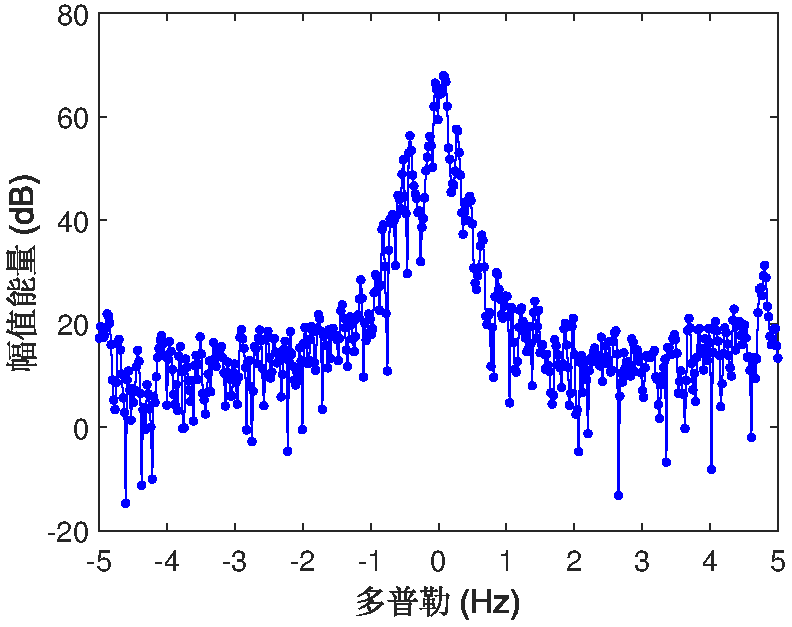
\includegraphics[width=6.67cm]{figures/othr/land}
		\label{fig:land}}
	\hfil
	\subfloat[海杂波频谱]{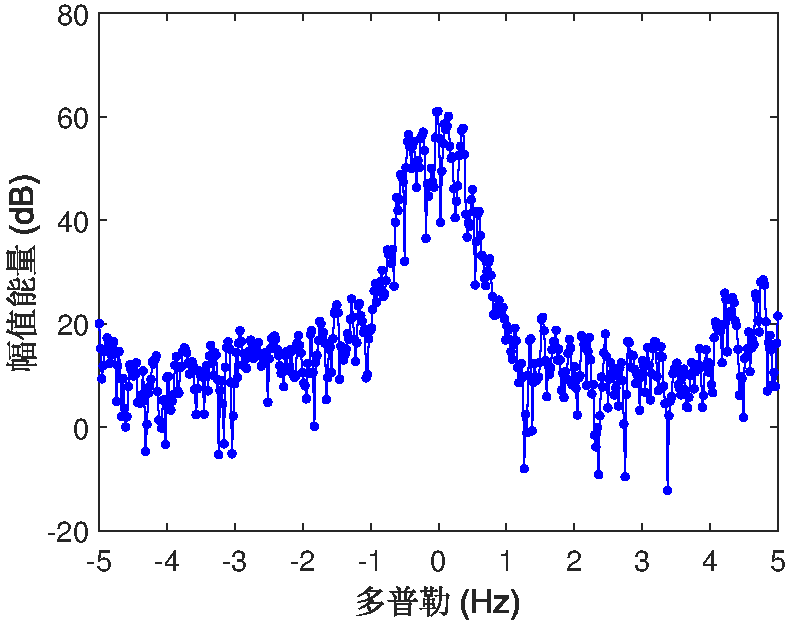
\includegraphics[width=6.67cm]{figures/othr/sea}
		\label{fig:sea}}
	\caption{两幅无法轻易区分的地海杂的频谱波示意图。图 \ref{fig:land} 作为地杂波最大幅值能量未处于零频处,图 \ref{fig:sea} 作为海杂波却无法容易的分辨出Bragg峰.}
	\label{fig:spectrum}
\end{figure}
%\vspace{-10pt}
本章选取了几种不同的雷达工作配置(工作频率、朝向等)下的数据,多普勒频率的范围可以是-5Hz至5Hz,也可以是-20Hz至20Hz。为了保证样本的多样性,本章对同一个雷达参数下的数据根据季节、地理位置、一天的早中午进行了选择,确保可以覆盖尽可能多的情形,图\ref{fig:classical_spectrum}展示了一些典型的频谱数据。
\begin{figure}[H]
	\centering
	\subfloat[杂波干扰严重的频谱图]{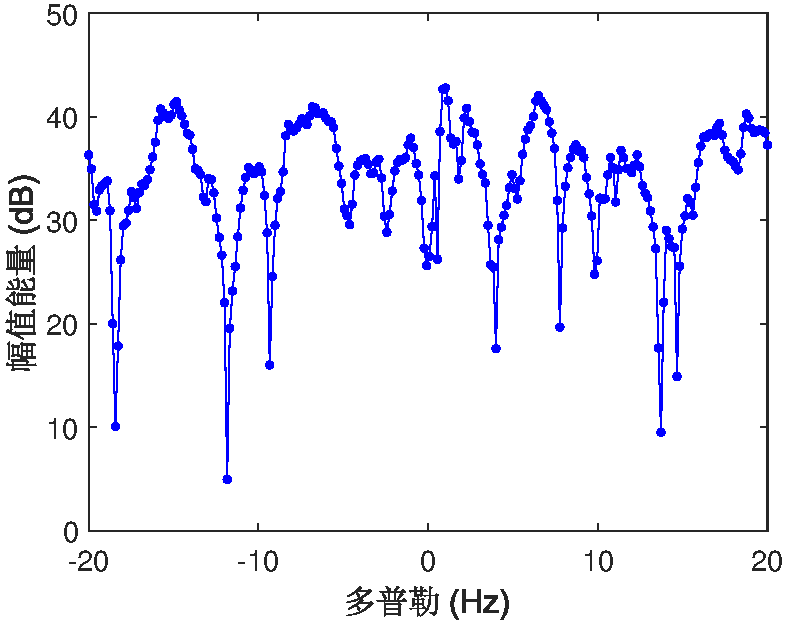
\includegraphics[width=6.67cm]{figures/othr/noise}}
	\hfil
	\subfloat[具有较强展宽的频谱图]{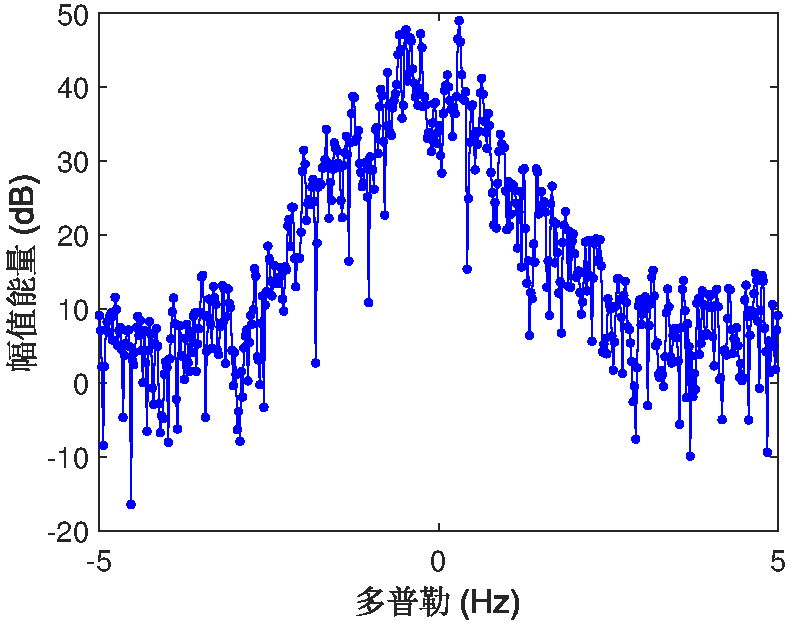
\includegraphics[width=6.67cm]{figures/othr/wide}}
\end{figure}
\begin{figure}[H]
	\centering
	\subfloat[Bragg峰缺失频谱图]{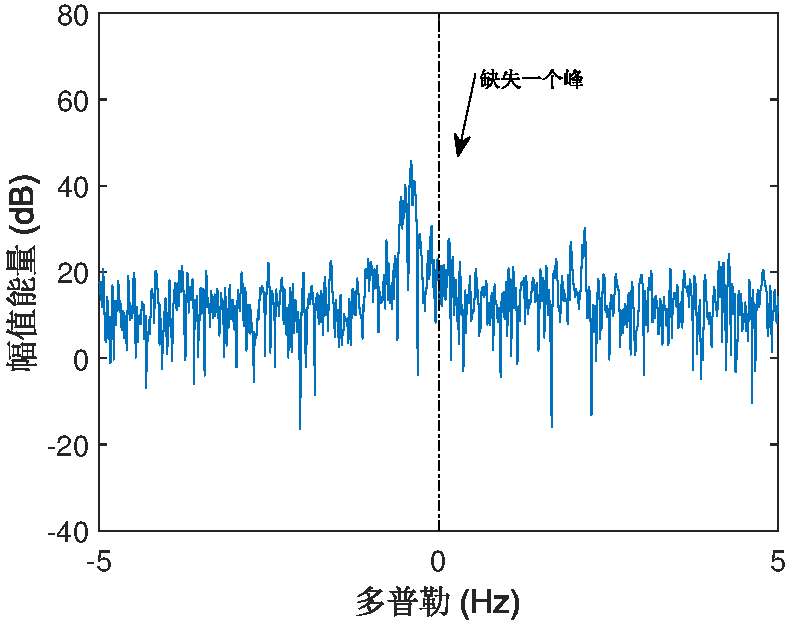
\includegraphics[width=6.67cm]{figures/othr/lost}}
	\hfil
	\subfloat[Bragg峰偏移频谱图]{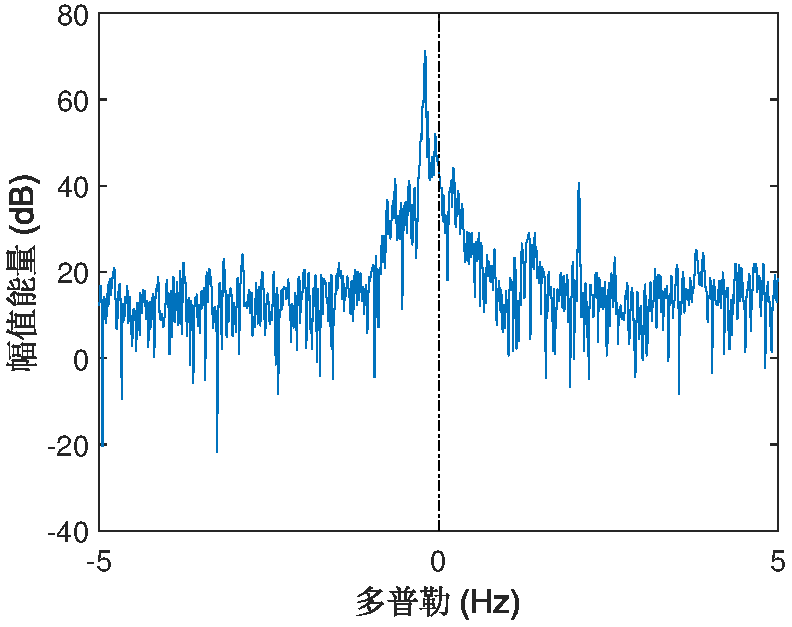
\includegraphics[width=6.67cm]{figures/othr/shift}}

	\subfloat[对空工作模式频谱图]{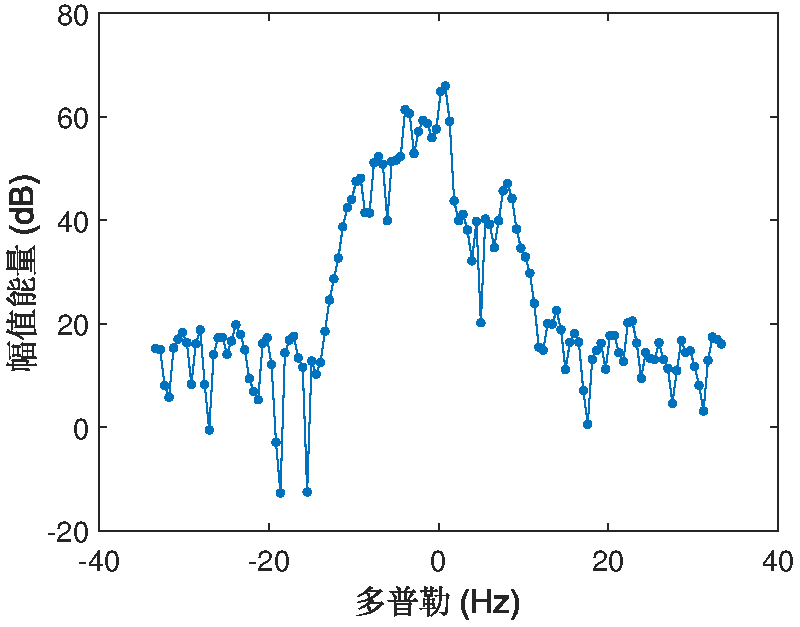
\includegraphics[width=6.67cm]{figures/othr/sky}}
	\hfil
	\subfloat[对海工作模式频谱图]{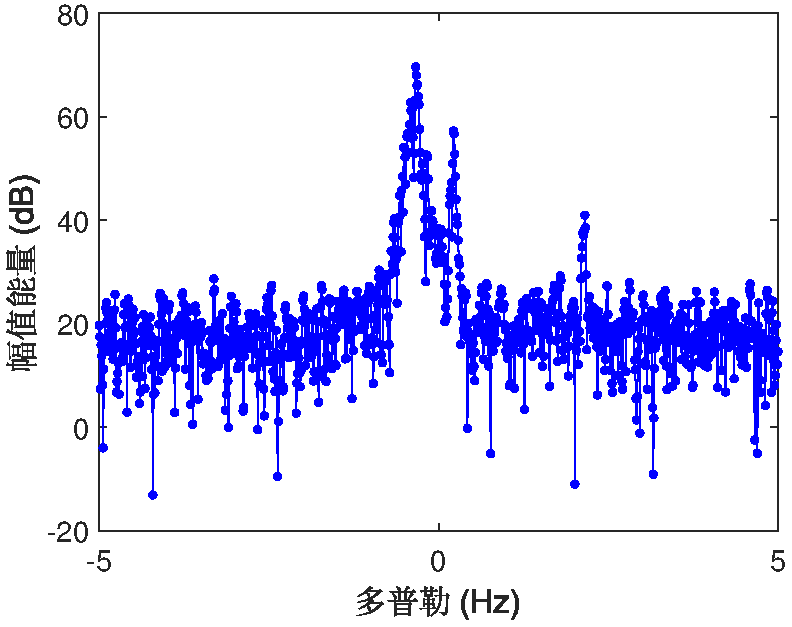
\includegraphics[width=6.67cm]{figures/othr/tosea}}
	\caption{复杂环境下频谱图}
	\label{fig:classical_spectrum}
\end{figure}


\subsection{数据集分组}
在本章的问题中,当雷达配置发生变化时,我们会获得不同的频率范围和精度频谱数据。
例如,一些频谱数据的频率变化范围为-5Hz到5Hz、具有512个相干积累点,而另一些数据的频率变化范围为-10Hz到10Hz、
相干积累点数为256个。因此,基于这两个条件,将所有数据分为4组:
\begin{itemize}
	\item 组 A: 如图\ref{fig:case128}所示,具有128个相干积累点数,频率变化范围为-5Hz到5Hz。
	\item 组 B: 如图\ref{fig:case256}所示,具有256个相干积累点数,频率变化范围为-5Hz到5Hz。
	\item 组 C: 如图\ref{fig:case512}所示,具有512个相干积累点数,频率变化范围为-5Hz到5Hz。
	\item 组 D: 如图\ref{fig:case1024}所示,具有1024个相干积累点数,频率变化范围为-5Hz到5Hz。
\end{itemize}
本章只选择了上述四个具有典型意义的分组的数据(如图\ref{fig:group}所示)来进行验证,舍弃了其余类型的与他们相似的数据,例如频率变化范围为-10Hz到10Hz的具有512个相干积累点的数据,这与组B的数据基本相同。同时,通过人工辨识的方法从中抽取出可以准确判定为地或者海的样本数据用于实验的训练和测试。
\begin{figure}[hbt]
	\centering
	\subfloat[组 A]{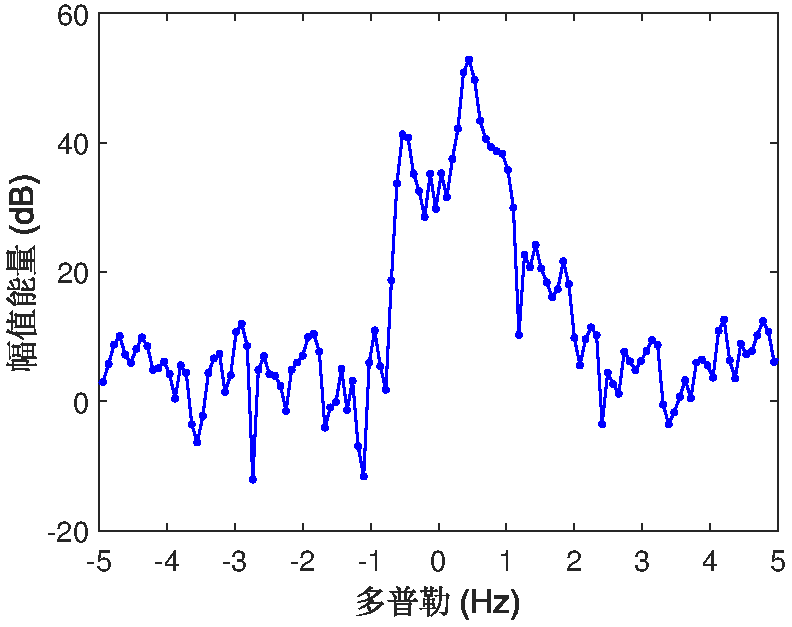
\includegraphics[width=6.67cm]{figures/othr/group128}
		\label{fig:case128}}
	\hfil
	\subfloat[组 B]{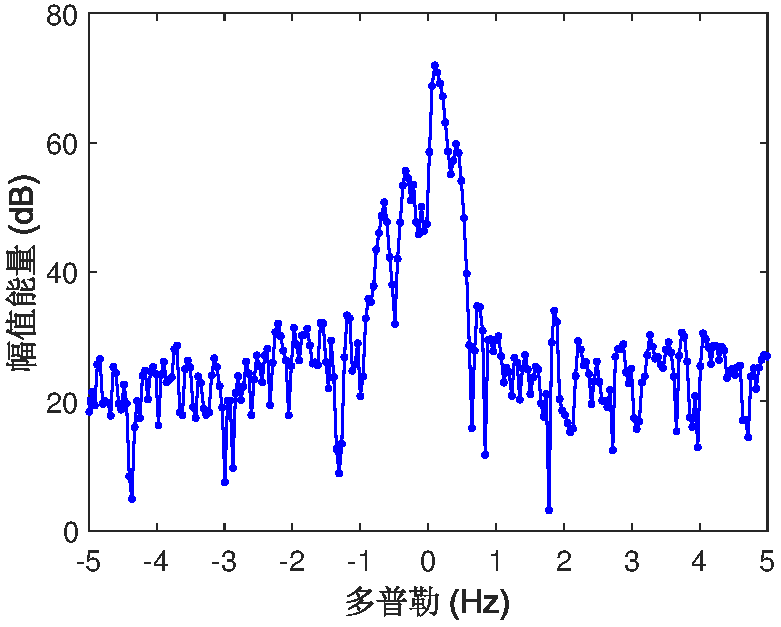
\includegraphics[width=6.67cm]{figures/othr/group256}
		\label{fig:case256}}

	\subfloat[组 C]{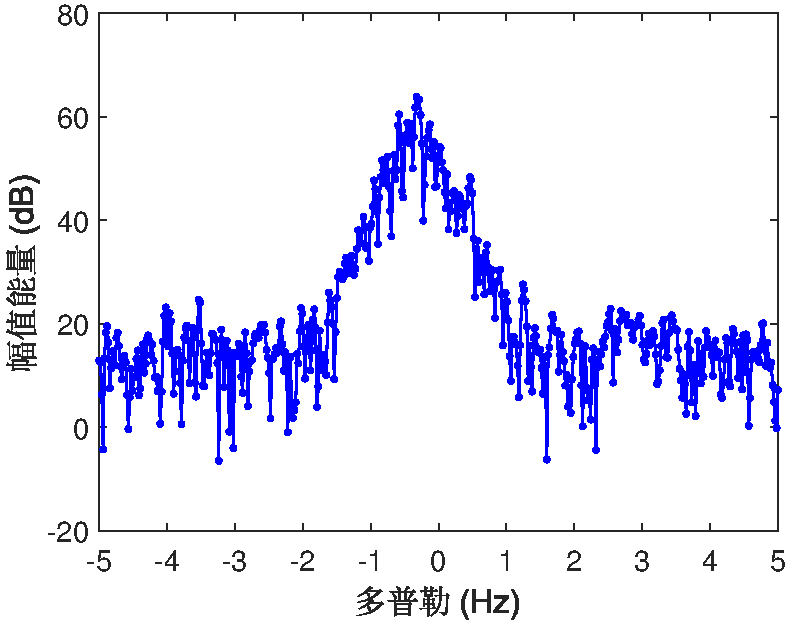
\includegraphics[width=6.67cm]{figures/othr/group512}
		\label{fig:case512}}
	\hfil
	\subfloat[组 D]{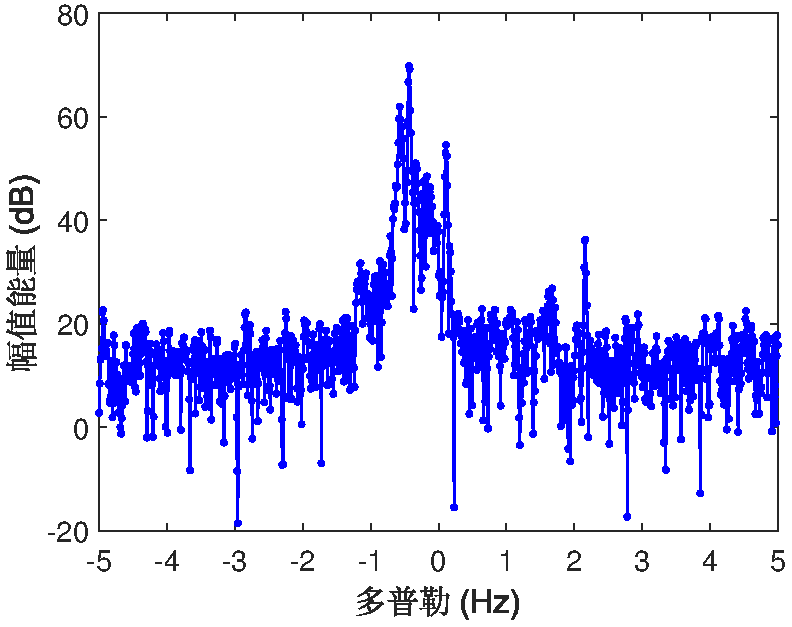
\includegraphics[width=6.67cm]{figures/othr/group1024}
		\label{fig:case1024}}
	\caption{不同组数据的频谱对比示意图}
	\label{fig:group}
\end{figure}

\section{地海杂波识别算法}
\label{sec:othr_cnn}
天波雷达目标的坐标配准问题在很大程度上影响了其定位精度,特别是电离层参数无法准确及时获得的较远区域。识别地海分界线主要有两个优点:第一个是可以使用获取的杂波地形图与实际的地图进行匹配,然后根据匹配结果计算偏移量,得到坐标修正系数,用来提高目标定位精度;另一方面,可以利用由识别结果获得的频谱上的偏移来校正频谱本身,以提高目标检测概率和准确度。

如图\ref{fig:system}所示,天波雷达地海杂波识别技术的处理流程可分为信息预处理和地海杂波识别两个处理层。
具体过程为:对输入频谱数据进行清洗、裁剪、融合等预处理操作,根据频谱数据的特性进行相关积累点数匹配和多普勒频率范围匹配选择恰当的深度卷积神经网络分类器,然后将预处理过的整体频谱数据输入到分类器中,输出地海杂波识别结果。
\begin{figure}[hbt]
	\centering
	% 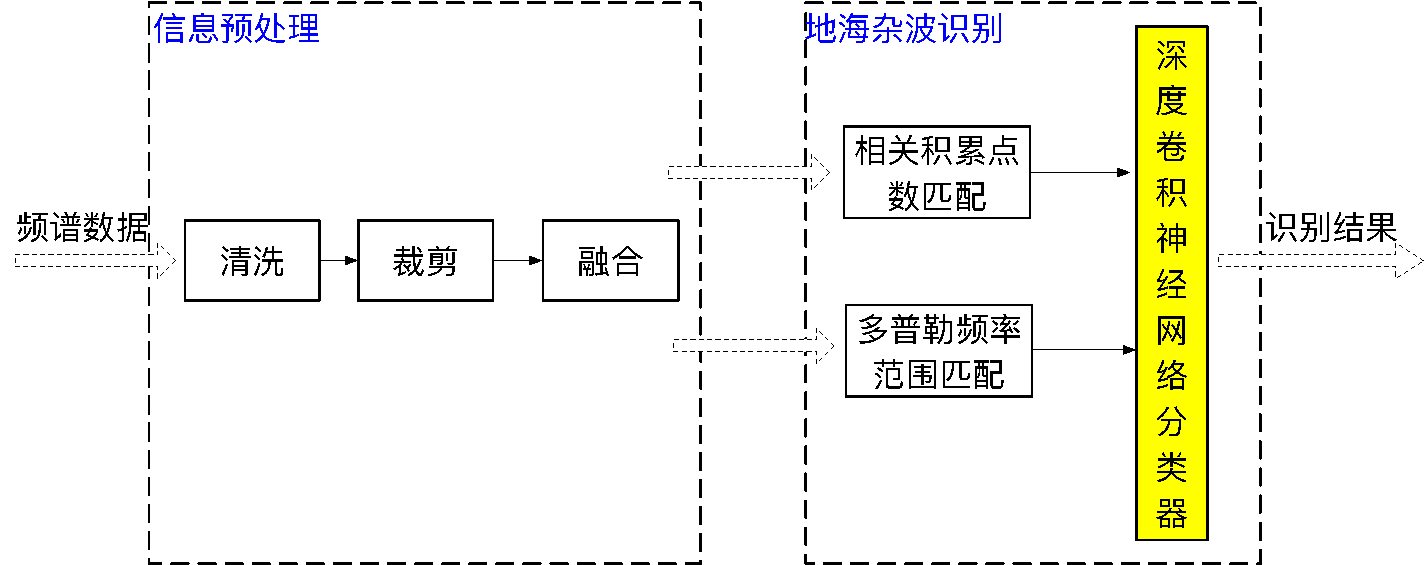
\includegraphics[width=13.5cm]{figures/othr/system}
	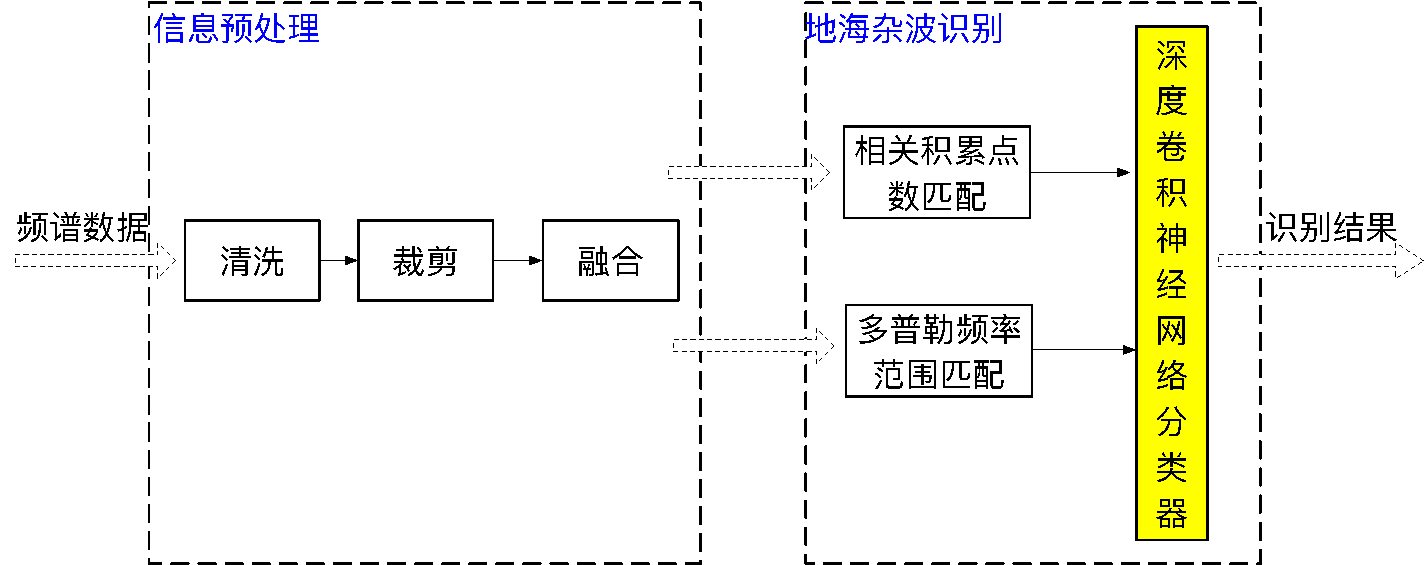
\includegraphics[width=\textwidth]{figures/othr/system}
	\caption{系统结构图}
	\label{fig:system}
\end{figure}

\subsection{数据预处理}

本章不同于传统分类问题中利用各种不同的由原始数据变换得到的特征,而是直接利用原始的杂波频谱数据来做地海杂波的识别。
同时针对地海杂波识别问题的数据形式,本章对输入数据做了二次处理。
本章并没有选择某距离方位角单元的完整杂波频谱数据作为输入特征,而是考虑到用来区分地海杂波属性的特征主要集中于零频附近,因此对原始频谱数据做了剪切处理,只选择了零频附近一个区域的数据。通过减少大量无用数据,在一定程度上减少了计算量而且有助于防止过拟合现象的出现。

另一方面,最初从雷达得到的数据为对时域数据进行快速傅立叶变换后获得的频域中的数据,本章对这些数据进行平移操作,将快速傅立叶变换的直流分量移到频谱中心。虽然,表面上看利用平移前后的数据训练和测试区别不大。然而,在实际的情况中,在经过平移变换后,频域数据的特征更加集中,这样在执行卷积运算时学习得到的特征也更加准确。
\begin{figure}[hbt]
	\centering
	\subfloat[原始频率能量曲线]{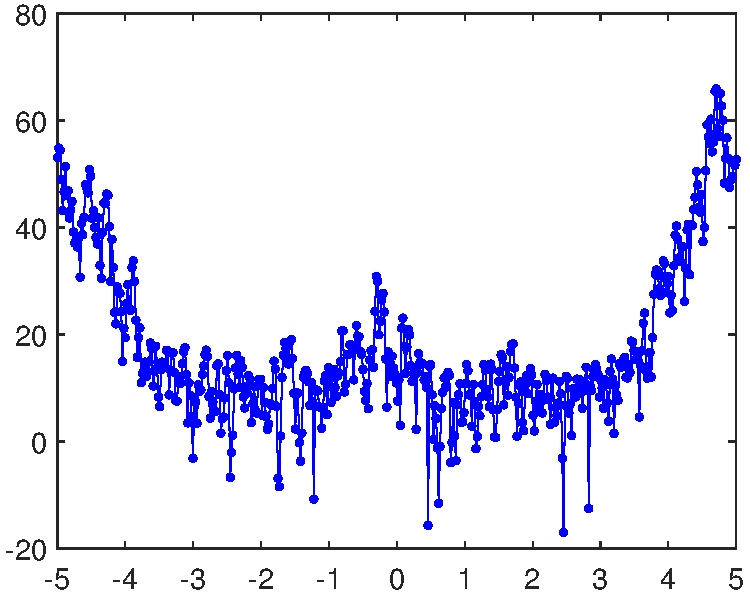
\includegraphics[width=6.67cm]{figures/othr/before_fft}
		\label{fig:before_fft}}
	\hfil
	\subfloat[经过频率平移的频率能量曲线]{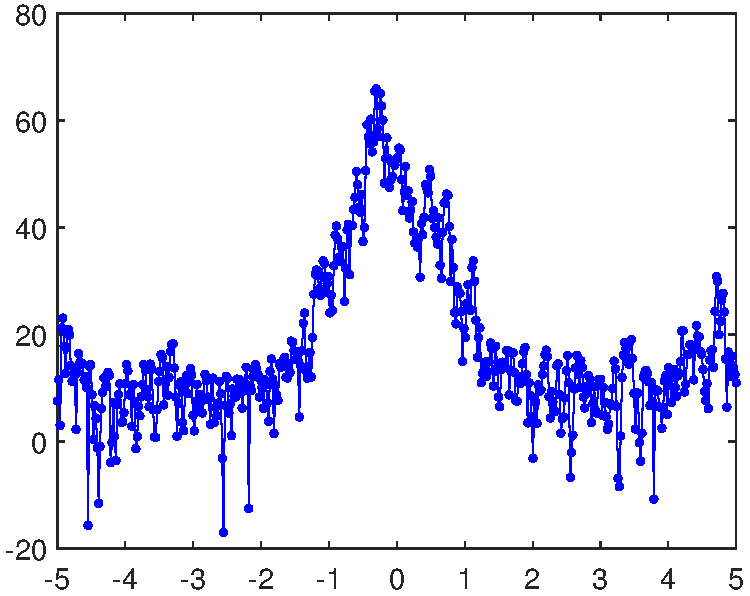
\includegraphics[width=6.67cm]{figures/othr/after_fft}
		\label{fig:after_fft}}

	\caption{频谱数据平移变换示意图}
	\label{fig:fft}
\end{figure}

频谱数据预处理频谱数据是从天波雷达获取的多普勒频率与幅度值对应的数据。在利用数据之前,首先对该数据进行清洗,
把图\ref{fig:delete}这种并非处于正常探测模式下的数据去除。

由于数据来自不同波位、不同时刻,具有不同的雷达工作频率,本章在利用这些数据进行训练或者识别前需要首先对其进行处理,主要包括将数据按照积累点数、波位和多普勒频率范围进行分类,不同类别的数据分开处理。
另一方面,由于地海杂波特征主要集中于多普勒频率较低的区域,可以将数据进行裁剪,只选取有效数据(本章在权衡信息保留以及计算量的情况下,保留了频率范围为$[-5\text{Hz},+5\text{Hz}]$的区域),在一定程度上减小计算量。
\begin{figure}[hbt]
	\centering
	\begin{minipage}{7cm}
		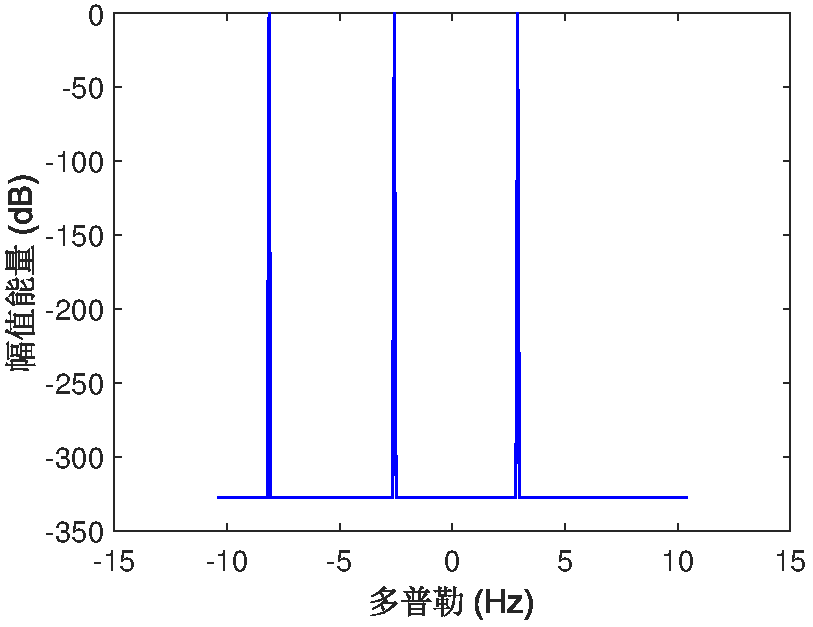
\includegraphics[width=6.67cm]{figures/othr/delete}
		\caption{需要被清洗掉的数据}
		\label{fig:delete}

	\end{minipage}
	\hspace{10pt}
	\begin{minipage}{7cm}
		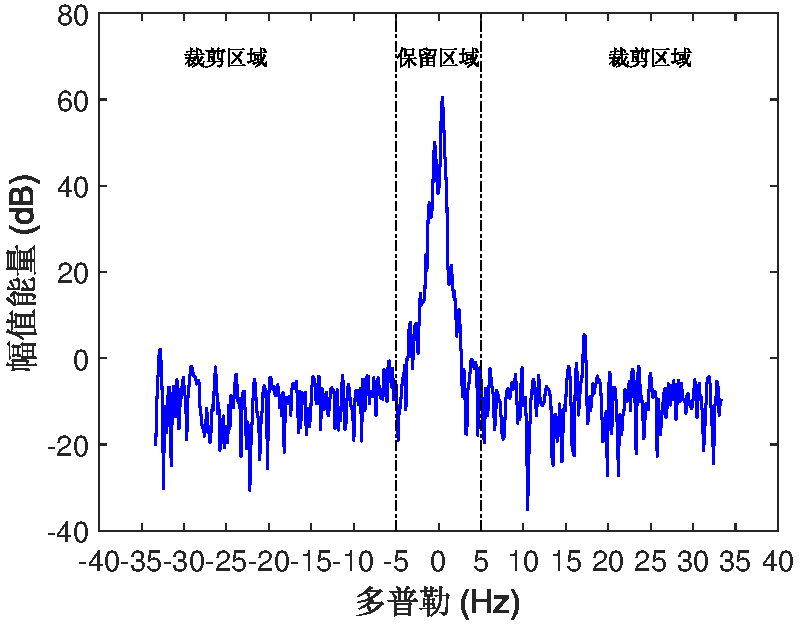
\includegraphics[width=6.67cm]{figures/othr/cut}
		\caption{数据裁剪示意图}
		\label{fig:cut}

	\end{minipage}

\end{figure}

受电离层非平稳、时变等特性影响,天波雷达杂波数据可能会出现较大波动。对这种波动不加处理会导致地海杂波识别结果不准确。在一个相对短时间内,电离层会保持一个较平稳的状态,也即同一距离方位单元的真实的地海属性不会发生变化。因此,本章采用滑窗融合的方法对输入数据进行预处理。其主要思想是将连续窗长时间$N$ 内的相邻杂波数据$x_1,x_2,\dots,x_N$ 加权融合得到新的频谱数据作为深度卷积神经网络分类器的输入:
\begin{equation}
	x=\sum_{i=1}^N w_ix_i,
	\label{equ:window_fusion}
\end{equation}
其中$w_i$ 为频谱数据$x_i$ 的权重,后面仿真验证小节详细讨论了窗长及权重的选择。从图\ref{fig:spectrum_fusion}可以看出,融合后的毛刺明显变少,更利于最终的分类识别。

\begin{figure}[hbt]
	\centering
	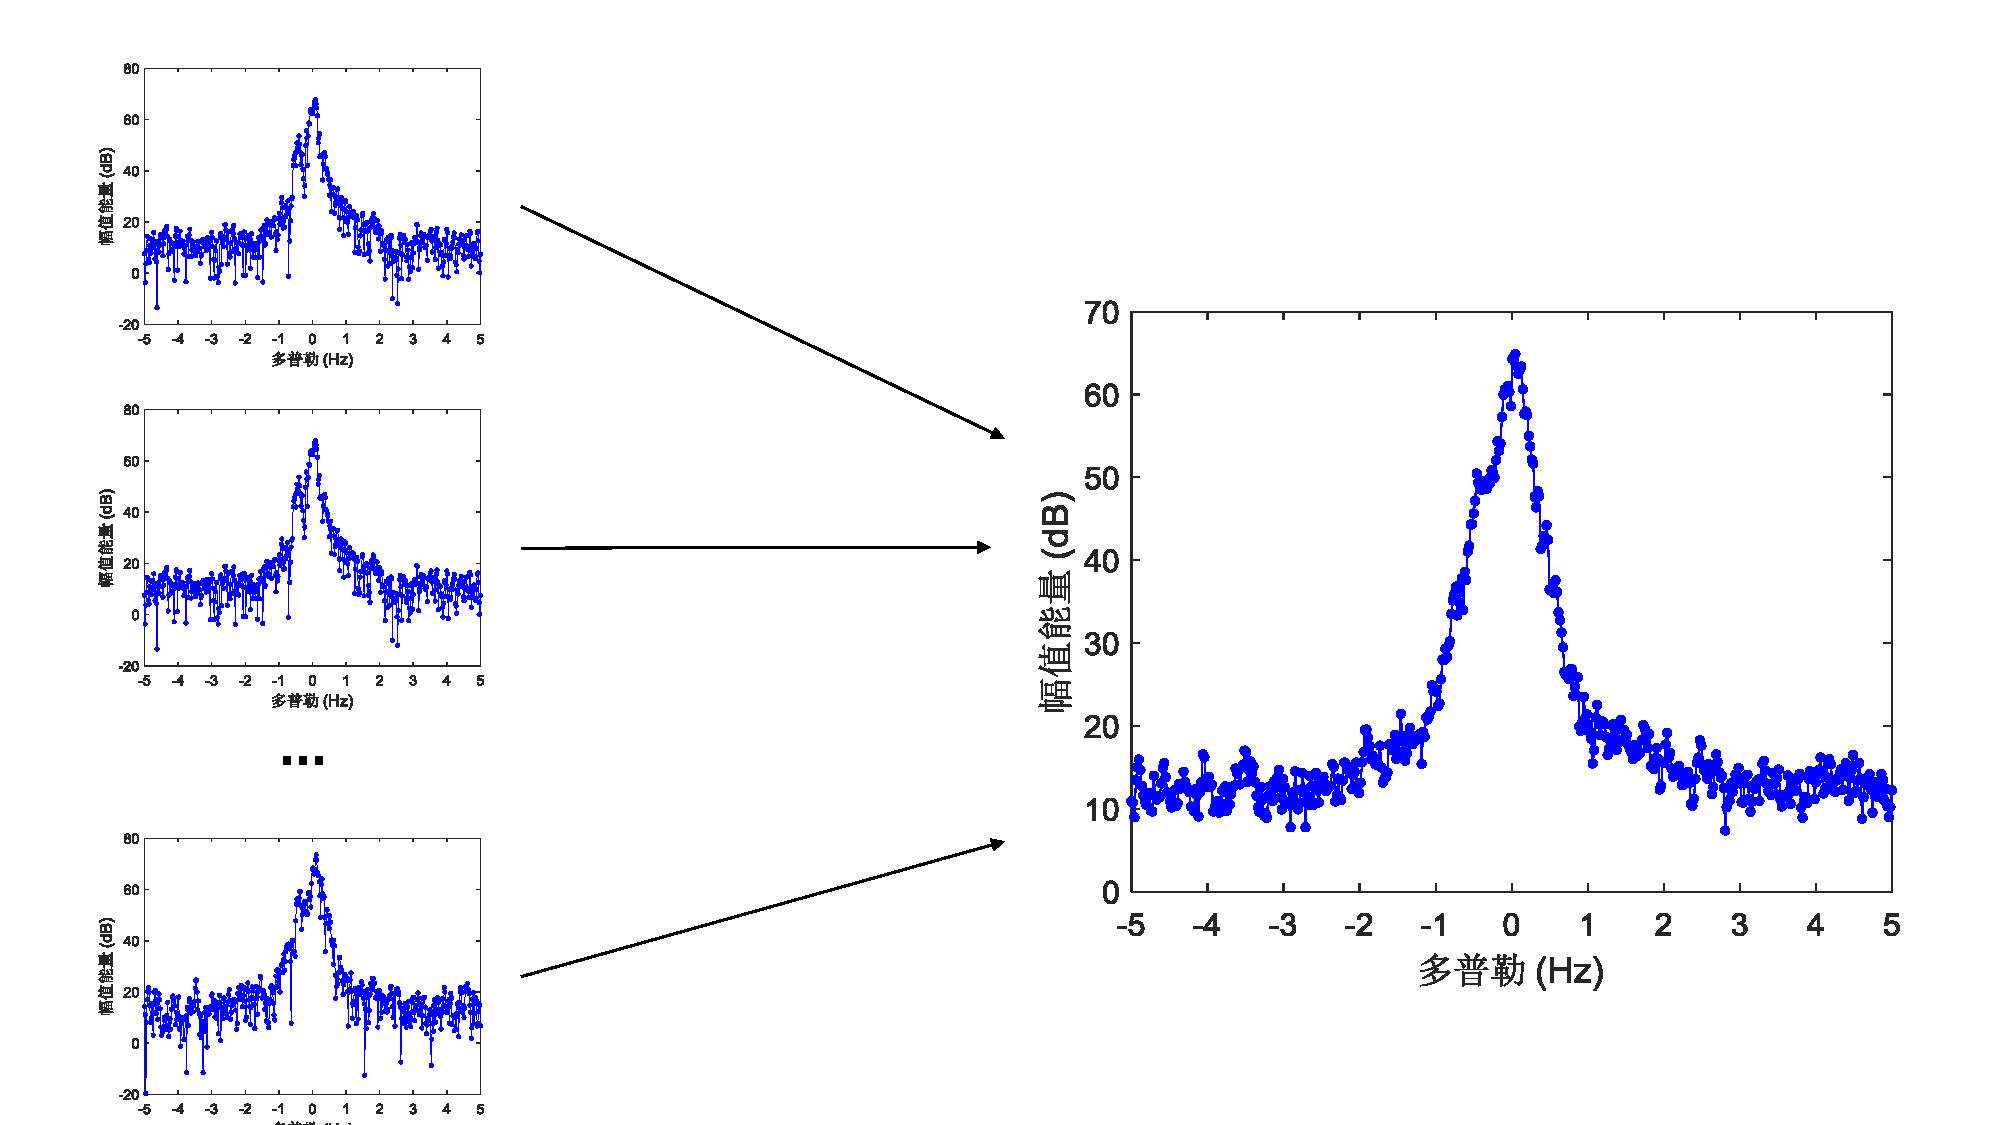
\includegraphics[width=13.5cm]{figures/othr/spectrum_fusion}
	\caption{数据融合示意图}
	\label{fig:spectrum_fusion}
\end{figure}

\subsection{分类算法设计}
深度学习体系结构中有几个网络模型,其中的卷积神经网络可以直接将整个需要分类的数据作为网络的输入,避免了传统识别算法中复杂的特征提取和数据重建过程。基于此优点,使卷积神经网络在本章所需解决的天波雷达地海杂波特征识别问题中有着巨大优势。
本章利用深度学习中的深度卷积神经网络算法,避免了地海杂波建模,从根本上克服了传统方法所面对的困难。如图 \ref{fig:othr_tech} 所示,其主要可分为训练和识别两个步骤:利用大量已打好标签的样本训练深度卷积神经网络;利用模型对新得到的雷达频谱数据进行识别,获得当前频谱数据的识别结果。

\begin{figure}[hbt]
	\centering
	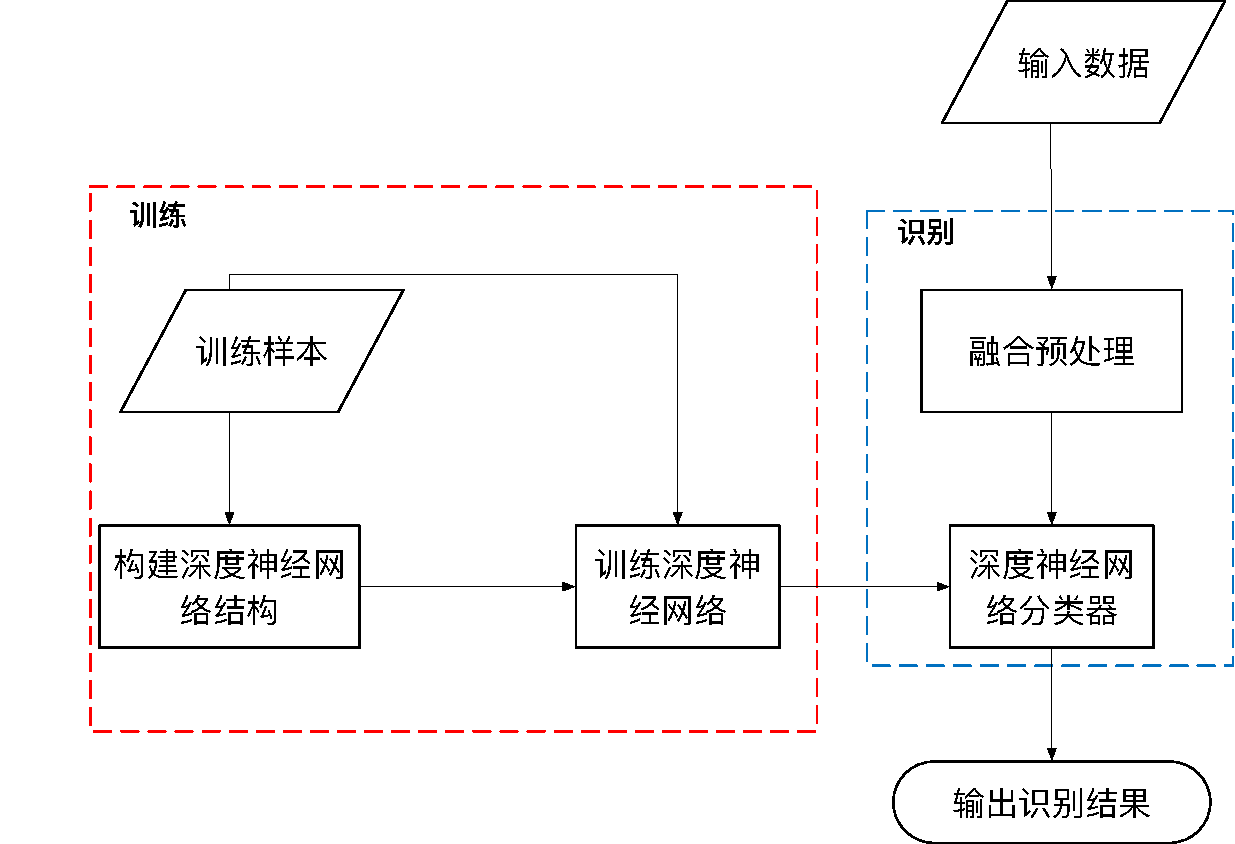
\includegraphics[width=9cm]{figures/othr/othr_tech}
	\caption{地海杂波识别算法结构图}
	\label{fig:othr_tech}
\end{figure}

利用深度卷积神经网络进行天波雷达地海杂波识别的主要挑战与难点在于网络模型的设计。典型的卷积神经网络由深层结构堆叠在一起的多个不同的层组成:输入层,多组卷积和池化层,有限数量的完全连接的隐层,以及输出层。
如图\ref{fig:fullconnect}所示,本章设计的深度卷积神经网络的结构在功能上可以分为特征提取和全连接网络这两部分,特征提取层主要通过卷积操作和池化操作从输入的频谱数据中学习出最好的卷积核以及这些卷积核的组合方式,同时每一层的输出又作为下一层的输入,每层具有多个特征向量,每个特征向量具有多个神经元,并且每个特征向量来自于一种卷积核所提取输入的一种特征;全连接网络,主要是将任何一个神经元均和上一层的任何神经元之间建立管理,通过矩阵运算得到输出结果。
\begin{figure}[hbt]
	\centering
	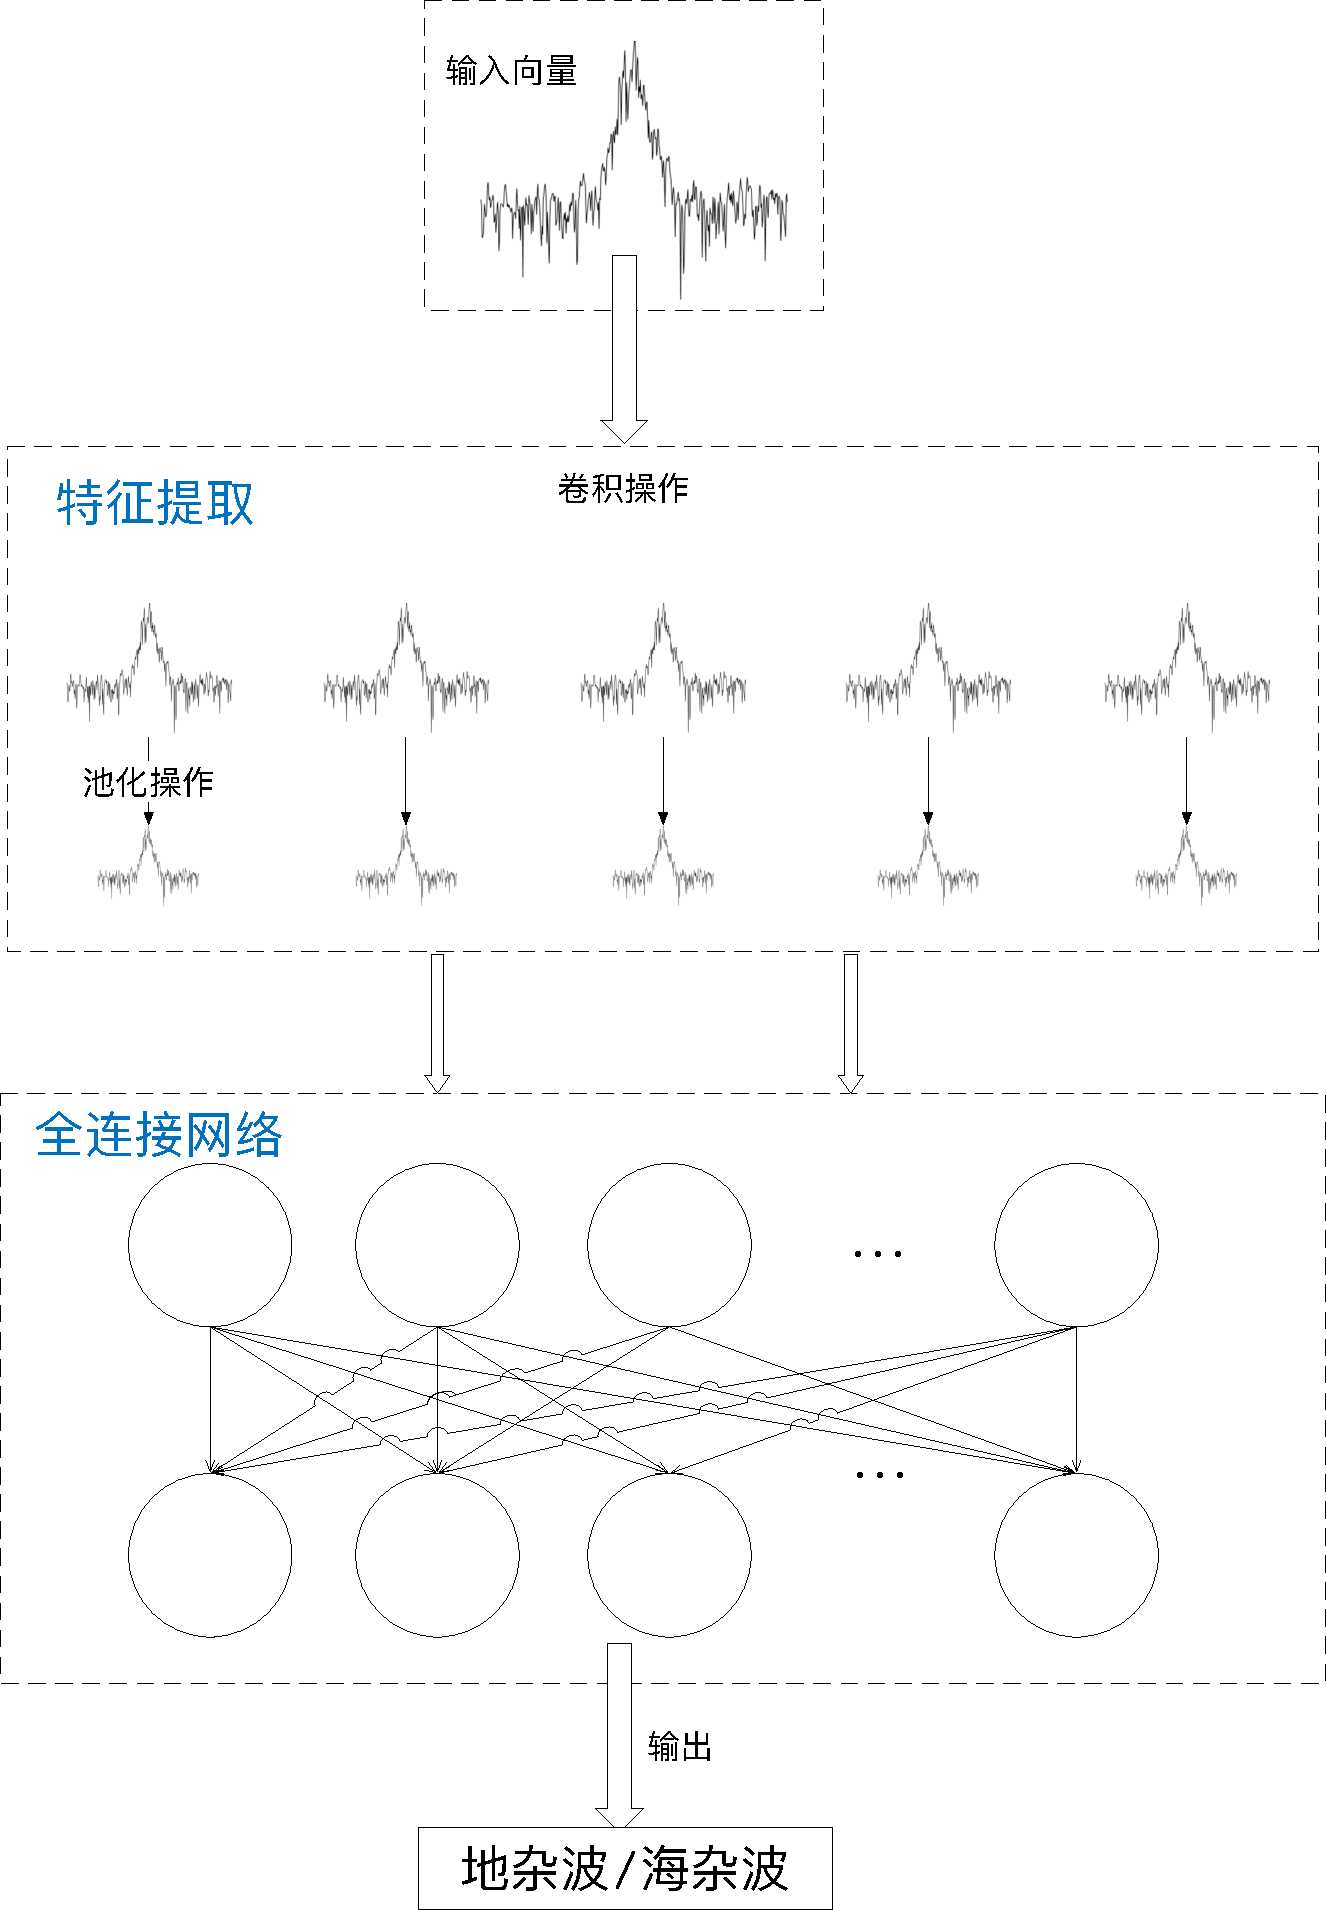
\includegraphics[width=6.67cm]{figures/othr/fullconnect}
	\caption{特征提取和全连接网络}
	\label{fig:fullconnect}
\end{figure}

本章的地海杂波识别问题主要是基于频谱数据的特征来识别。人工识别主要基于海杂波中存在关于零频对称的Bragg峰,而地杂波只存在零频率附近的一个峰值。然而,还有一些无法直观的描述的特征,如整体幅度等等。此外,在一些频谱数据中仍然有一些无用的特征,例如,出现一个目标,这部分可以通过卷积特征提取和权重共享容易地去除对最终识别的影响。因此,这种基于深度卷积神经网络的方法很适合本章的问题。

利用CNN进行地海杂波识别避免了对天波雷达回波的建模,从根本上避免了传统方法所面临的困难。本章根据地海杂波频谱数据以及其反映出来的特性,构建了一个具有六层的深度卷积神经网络,如图\ref{fig:struct}所示,每层从提取输入的卷积滤波器的特征导出多个特征向量,每个特征向量具有多个神经元。构建神经网络结构的基本步骤为:

步骤1:输入地海杂波频谱数据(此处以大小为$1\times N$ 的输入序列为例),对其进行卷积运算,得到第一个卷积层。经过不同参数的试验对比结果,最终确定使用32个大小为$1\times 3$ 的卷积核,故特征向量中每个神经元与输入中的$1\times 3$ 的邻域相连,这样此卷积层中的特征大小就为$1\times (N-3)$ 。又因为该卷积层有128个可训练参数(每个滤波器具有3个单元参数和一个偏置参数,一共32个滤波器,共$(1\times 3 + 1) = 128$ 个参数),共$128\times(N-3)$ 个连接,将连接通过ReLU激活函数。

步骤2:对卷积层进行最大池化处理,该操作采用一个特征代替相邻的多个特征。通过降低特征向量的长度,在减小了计算量的同时也在一定程度上修正了过拟合情形。

步骤3:将经过上述两个步骤获得的特征向量作为新的输入,重复三次步骤1至2,可以得到一个六层深度卷积神经网络结构。通过上述多阶段卷积操作,输入向量的特征获得了充分的提取。

步骤4:构建输出层。压平步骤3获得的特征向量,把多维的输入一维化,以此作为卷积层到全连接层的一个过渡。在第一个全连接层的基础上添加dropout参数,然后添加第二层全连接并通过激活函数Sigmoid,输出识别结果。

\begin{figure}[hbt]
	\centering
	% 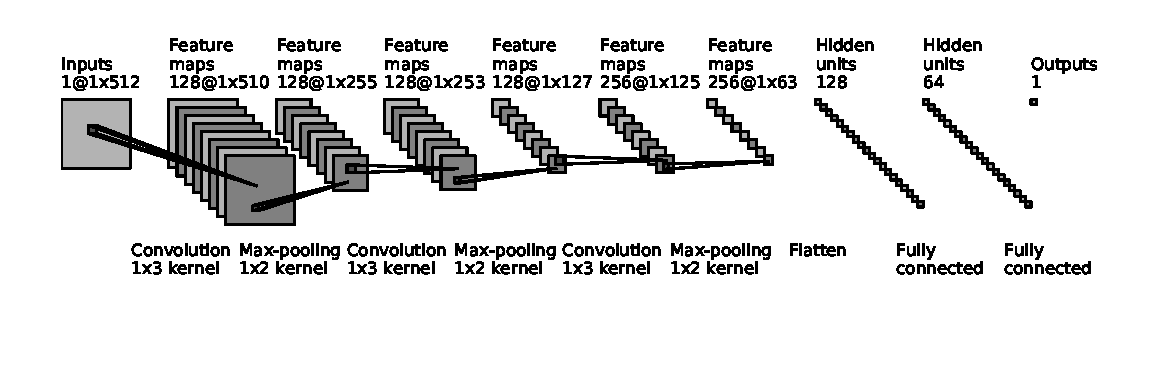
\includegraphics[width=13.5cm]{figures/othr/struct}
	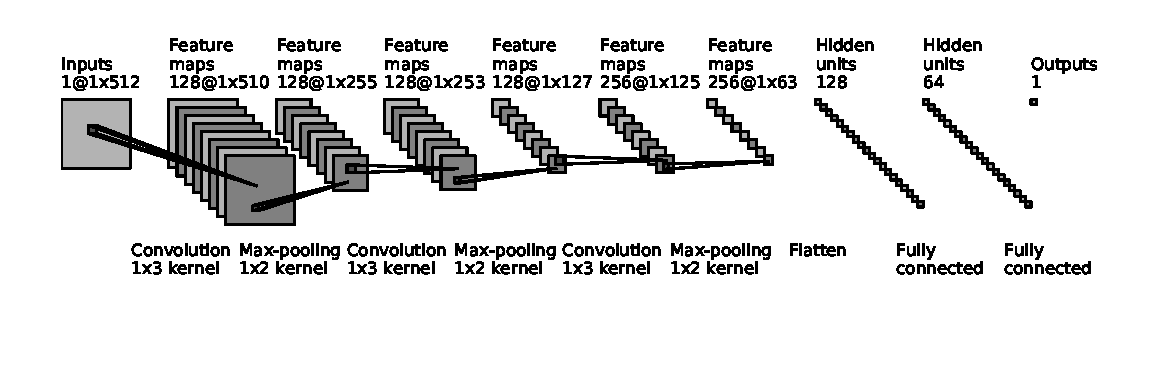
\includegraphics[width=\textwidth]{figures/othr/struct}
	\caption{卷积神经网络结构}
	\label{fig:struct}
\end{figure}

\subsubsection{训练算法}
在搭建好合理的深度神经网络结构之后,下一步需要利用大量的数据对该网络进行。
地海杂波识别问题由于分开训练不同相干积累点数和多普勒频率范围的数据,故首先需要对不同的数据进行分类处理并标注其地海杂波类型,通过此步骤完成训练样本的生成。接下来就是利用训练样本对搭建好的网络结构进行训练,获得最终的分类器。训练过程或者说学习过程主要是利用了梯度下降算法,梯度反映了参数的移动方向。这其中一个很重要的问题就是学习率的选择,学习率过小则运行缓慢,过大则无法得到很好的结果。

传统的神经网络优化方法是随机梯度下降,通过计算每次迭代的梯度更新参数。
然而,这种方法有两个缺点:一个是学习率的选择比较困难,因为它对所有参数使用相同的学习率,故很难选择一个很合适的初值;另一个是趋向于收敛到局部最优。

本章不仅考虑梯度,同时考虑包含梯度变化的信息,采用了一种具有自适应学习率的优化算法Adam(Adaptive Moment Estimation)。该算法利用梯度的一阶矩估计和二阶矩估计动态地调整每个参数的学习率。经过偏置校正后,每一次迭代学习率都有明确范围,使得参数更加平稳。
传统的梯度下降更新规则为$\theta \leftarrow \theta'=\theta-\eta\nabla C$ ,$\theta$ 表示需要学习的参数,$\eta$ 为学习速率,$\nabla C$ 为损失函数的梯度,则变为:
\begin{align}
	v\leftarrow v'=\mu v - \eta \nabla C \\
	\theta \leftarrow \theta' = \theta +v',
\end{align}
其中,$\mu$ 是用来控制梯度变化的超参数。据此可以得到算法流程\ref{tab:Adam}。

\begin{algorithm}[hbt]
	\caption{Adam 训练算法}
	\label{tab:Adam}
	\begin{algorithmic}[1] %每行显示行号
		\Require 训练样本$X$,样本标签$Y$,最大迭代次数$K$,步长$\varepsilon$,初始目标参数$\theta$
		\Ensure 学习后的参数$\theta$
		\State 初始化矩估计的期望衰变率$\rho_1=0.9,\rho_2=0.999$,一阶矩与二阶矩变量$s=0,r=0$,迭代次数$k=0$
		\While{$k < K$}
			\State 从训练集中获取对应于目标$y^{(i)}$ 的$m$ 个采样样本 $\{x^{(1),\dots,x^{(m)}}\}$ ,其中$m$ 为批处理中一批样本的个数。
			\label{line:start}
			\State 计算梯度$g \leftarrow \frac{1}{m} \nabla_{\theta} \sum_i L(f(x^{(i)};\theta), y^{(i)}) $,其中$L$为对数损失函数,其定义为$L(P(Y|X),Y) = - \log P(Y|X) $。
			\State 更新迭代次数$k \leftarrow k+1 $
			\State 更新有偏一阶矩估计$s \leftarrow \rho_1 s + (1 - \rho_1) g $,有偏二阶矩估计$r \leftarrow \rho_2 r + (1-\rho_2) g \odot g $,其中$ g \odot g $表示对应元素的乘积。
			\State 修正一阶矩估计$\hat{s} \leftarrow \frac{s}{1-\rho^k_1} $,二阶矩估计$\hat{r} \leftarrow \frac{r}{1-\rho^k_2} $。
			\State 更新参数 $\theta \leftarrow \theta + \Delta \theta = \theta - \varepsilon \frac{\hat{s}}{\sqrt{\hat{r}} + \delta} $
			,其中$\delta = 10^{-8} $
			用来保持稳定性。
		\EndWhile
	\end{algorithmic}
\end{algorithm}

针对地海杂波识别这个二分类问题,选择逻辑损失函数来训练本章的模型:
\begin{equation}
	L(z_i) = log(1+e^{-z_i}),
\end{equation}
其中, $z_i=y_i(w^T x_i + b)$, $y_i$ 是采样样本 $x_i$的标签,其为1代表地杂波,0为海杂波。

\subsection{分类阈值设计}
分类器的输出结果为给定回波频谱数据来自于海洋或者陆地的概率,一般使用$ 0.5 $作为概率阈值来进行分类。
但是,结合海洋的变化远远大于陆地导致的海洋容易被误判为陆地以及海洋或者陆地均应该是连续的这两个实际情况,对分类的概率阈值进行了设计,这将在第\ref{sec:othr_experiment}节通过仿真实验进行讨论。
此外,还需要根据某距离方位单元周围单元的识别结果进行进一步处理。
也就是说,设初步结果为$y_{m,n}$,其中,$m$表示方位角的第$ m $ 个单元,$ n $表示第$ n $个径向距单元,那么,最终结果$y_{i, j}$可以表示为:
\begin{equation}
y_{i, j} = \sum_{m=1}^{M}\sum_{n=1}^{N}w_{m,n}\cdot y_{m,n},
\end{equation}
其中,$ w_{m,n} $是$(m,n)$单元处识别结果$y_{m,n}$的权重,$M$为利用的方位上区域单元的个数,$N$为利用的径向距上区域单元的个数。
\section{验证}
\label{sec:othr_experiment}
在本节中,本章利用相应数据评估了所提出的基于深度学习的地海杂波识别算法的性能,并与基于LMS\ucite{turley2013high}的根据多普勒频谱进行分类的算法和基于支持向量机进行分类的算法\ucite{jin2012svm}进行了对比。
\subsection{算法实现}
\subsubsection{基于LMS的算法}
该方法主要基于文献\cite{turley2013high},其主要思想是利用加权最小均方算法来求解区域的模糊度,其中区域模糊度的定义如下:
\begin{equation}
	f_D = f_I + f_{cur} + f_B\left\{
		\begin{array}{rcl}
		1/2       &      & \text{前向海}\\
		0     &      & \text{陆地}\\
		-1/2       &      & \text{后向海}
		\end{array} \right.
\end{equation}
其中, $f_B$ 是前向Bragg回波与后向之差,$f_I$ 和 $f_{cur}$分别是电离层动力过程和海流产生的多普勒频偏。
\subsubsection{基于SVM的方法}
参照文献\cite{jin2012svm},本章选择了如下三个特征作为分类器的特征向量:
\begin{itemize}
	\item 最大后向散射幅值,
	\item 频谱中最大与次大幅值频率之差,
	\item 频谱中最大与次大幅值幅度之差,
\end{itemize}
并利用网格搜索法对参数进行了调优。
为了确保有足够的数据来训练和测试,本章选取了不同的雷达工作条件、天气、时间的多组数据(每组约有20000个频谱数据),随机选择其中$70\%$的数据作为训练数据,$20\%$作为交叉验证数据,其他数据用作测试数据,该数据集同样被应用于基于深度卷积神经网络的分类器。
\subsubsection{算法参数设置}
根据图\ref{fig:struct}所示的结构搭建了深度卷积神经网络分类器。前两个卷积层具有32个滤波器,第三个卷积层有64个滤波器。全连接层添加dropout参数为0.5。利用Adam优化算法来训练网络,初始的学习率为0.001,学习迭代次数为20次。
\subsubsection{评估方法}
分类问题的算法性能评估指标主要是分类的准确度。然而,由于此处利用相应数据进行验证,这些数据没有准确的标签,尤其是地海交界处的杂波的类别更加难以确定。而在实际工程实践中,该部分的识别准确度影响着最终电离层参数的辨识。由于在实际的地图中可以得到地海交界处也即海岸线处的地理位置坐标,也即可以得到该区域的形状。
因此,本章设计了与地图的匹配程度的评估方法来分析不同识别算法海岸线部分杂波识别的性能,其定义如下:
\begin{equation}
g_{C_1, C_2} = \frac{area({C_1\cap C_2})}{\max(area({C_1}), area({C_2}))}
\end{equation}
用0和1来二值化地图区域,如图\ref{fig:binary}所示。$area(C)$表示区域$C$的面积, $g_{C_1, C_2}$表示区域$C_1$ 和 $C_2$ 的匹配度。
\begin{figure}[hbt]
	\centering
	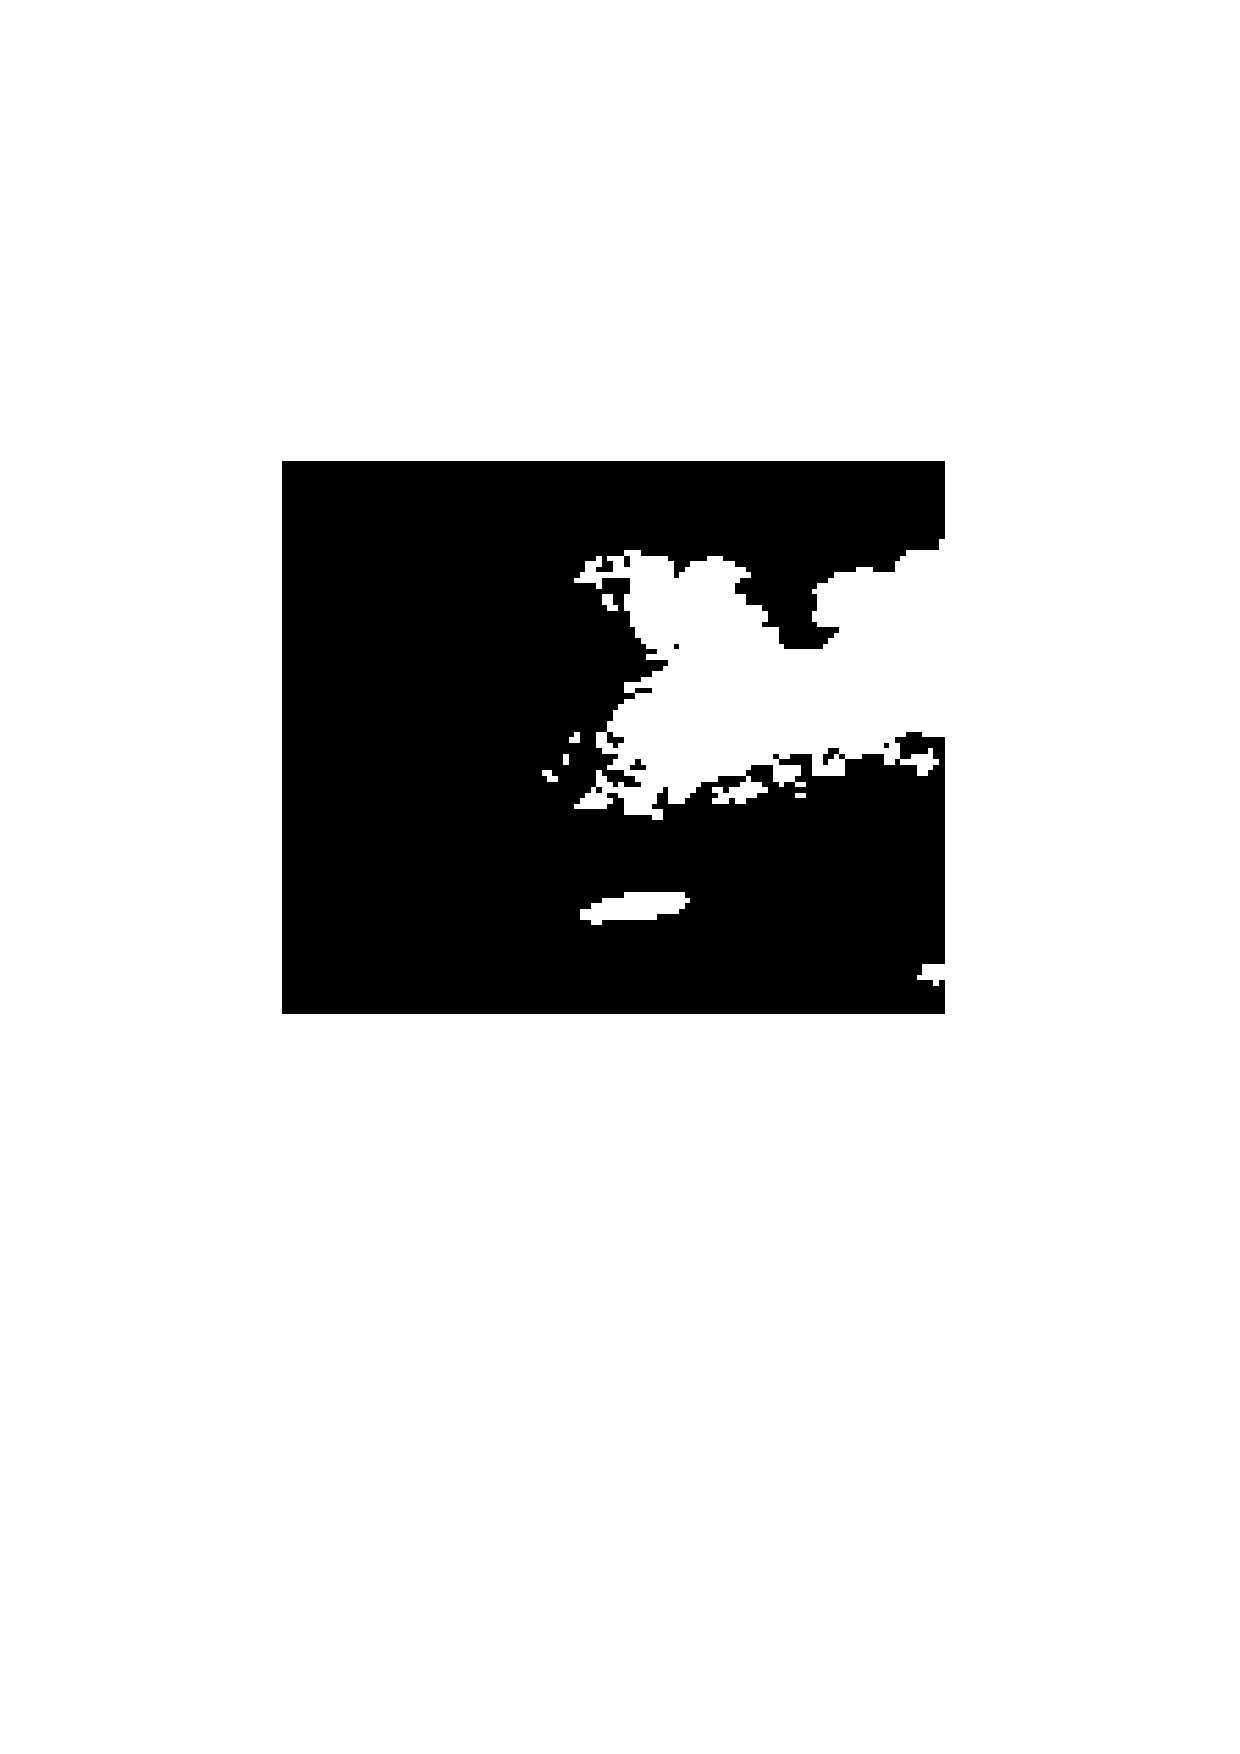
\includegraphics[width=6.67cm]{figures/othr/binary}
	\caption{二值化地图}
	\label{fig:binary}
\end{figure}
\subsection{仿真结果分析}
首先利用四组数据对三种算法进行对比分析,实验结果如表\ref{tab:methods}所示,
可以明显的看到,本章提出的基于CNN的算法的识别性能最好。
\begin{table}[H]
	\renewcommand{\arraystretch}{1.3}
	\caption{三种算法的识别精度对比}
	\label{tab:methods}
	\centering\sWuhao
	\begin{tabularx}{\textwidth}{>{\centering\arraybackslash}X>{\centering\arraybackslash}X>{\centering\arraybackslash}X>{\centering\arraybackslash}X}
		\toprule
		数据集 & CNN & SVM & LMS \\
		\midrule
		组 A  & 96.97\% & 85.69\% & 81.85\% \\
		组 B & 97.14\% & 88.57\% & 81.93\% \\
		组 C & 99.04\% & 89.03\% & 88.57\% \\
		组 D  & 99.69\% & 91.61\% & 90.33\% \\
		\bottomrule
	\end{tabularx}
\end{table}
选取CNN识别错误的结果进行分析,发现大部分识别错误的数据特征十分不明显,即使是人工也无法很准确地判定,如图 \ref{fig:error_result} 所示。

\begin{figure}[hbt]
	\centering
	\subfloat[地杂波被错误识别为海杂波]{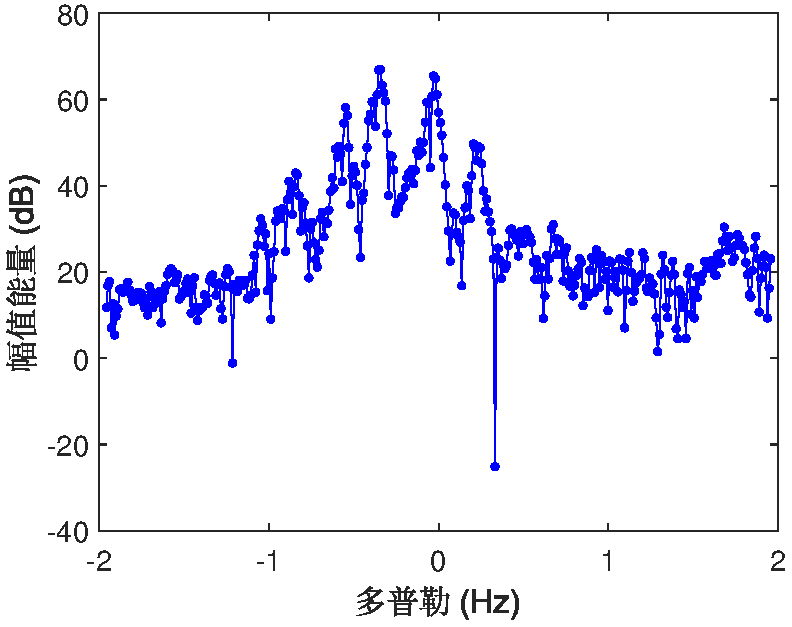
\includegraphics[width=6.67cm]{figures/othr/error_land}
		\label{fig:error_land}}
	\hfil
	\subfloat[海杂波被错误识别为地杂波]{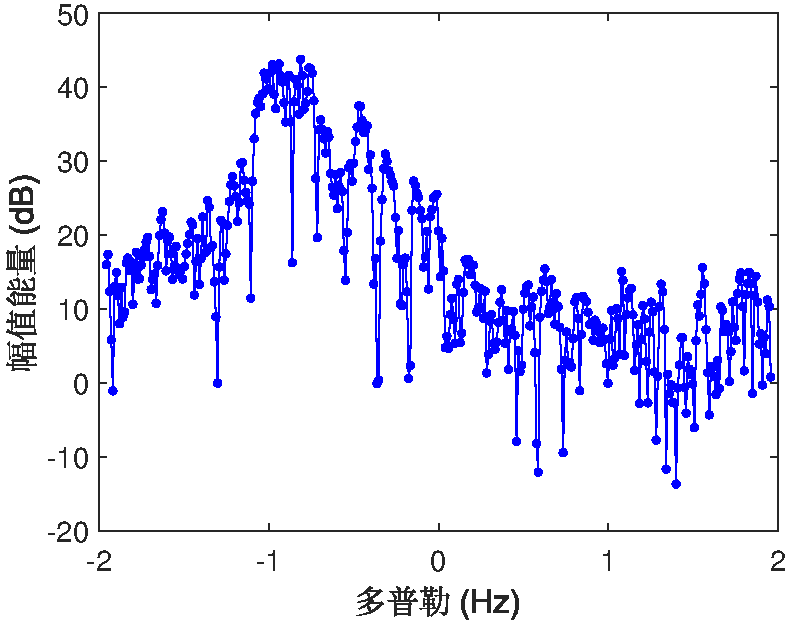
\includegraphics[width=6.67cm]{figures/othr/error_sea}
		\label{fig:error_sea}}
	\caption{识别错误的结果}
	\label{fig:error_result}
\end{figure}

由于数据集自身的一些限制条件,本章选择在组D所在的数据集进行了地图匹配度的比较实验。从表\ref{tab:method_pair}可以看出,基于CNN的算法在匹配度方面要远高于其余两种方法,证明了本章算法在地海边界处仍然可以保持很高的精度。
\begin{table}[H]
	\renewcommand{\arraystretch}{1.3}
	\caption{匹配度对比}
	\label{tab:method_pair}
	\centering\sWuhao
	\begin{tabularx}{\textwidth}{>{\centering\arraybackslash}X>{\centering\arraybackslash}X>{\centering\arraybackslash}X>{\centering\arraybackslash}X}
		\toprule
		& CNN & SVM & LMS \\
		\midrule
		匹配度 & 0.92 & 0.23 & 0.21 \\
		\bottomrule
	\end{tabularx}
\end{table}

为了验证迭代次数对本章基于深度卷积网络算法的影响,本章对不同组数据在不同迭代次数下进行了实验,结果如图\ref{fig:group_results}所示,结果表明本章提出的算法可以在不同的数据集组中均可以较快的收敛。
组A的数据集由于频率和相干累计点的比例最小导致其所包含特征最小,而需要较多的迭代次数。
图\ref{fig:sizes}表明即使在数据量很小的情况下,本章的算法仍保持着很高的准确率。

\begin{figure}[hbt]
	\centering
	\begin{minipage}{7cm}
		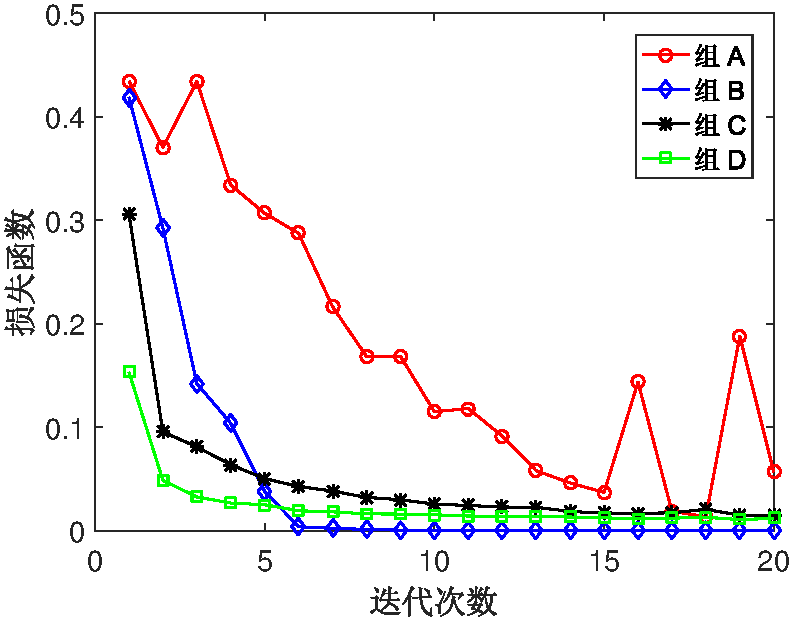
\includegraphics[width=6.67cm]{figures/othr/group_results}
		\caption{不同数据集损失函数随迭代次数变化图}
		\label{fig:group_results}
	\end{minipage}
	\hspace{10pt}
	\begin{minipage}{7cm}
		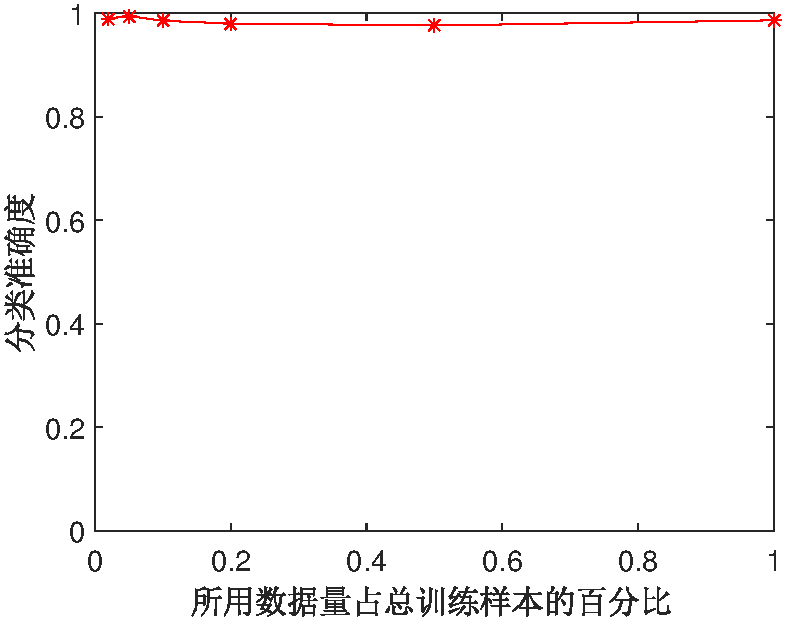
\includegraphics[width=6.67cm]{figures/othr/sizes}
		\caption{不同数量数据集的分类准确度曲线图}
		\label{fig:sizes}
	\end{minipage}

\end{figure}

由于卷积神经网络的参数对最终分类识别的准确率起着重要的作用,对参数的选择进行一些分析。
首先分析了批长度(Batch Size)和迭代次数变化时,验证集数据的分类准确度。
图\ref{fig:epoch}表明识别准确度随着迭代次数的增加而增长,而当批长度变大时,收敛速度加快。
\begin{figure}[hbt]
	\centering
	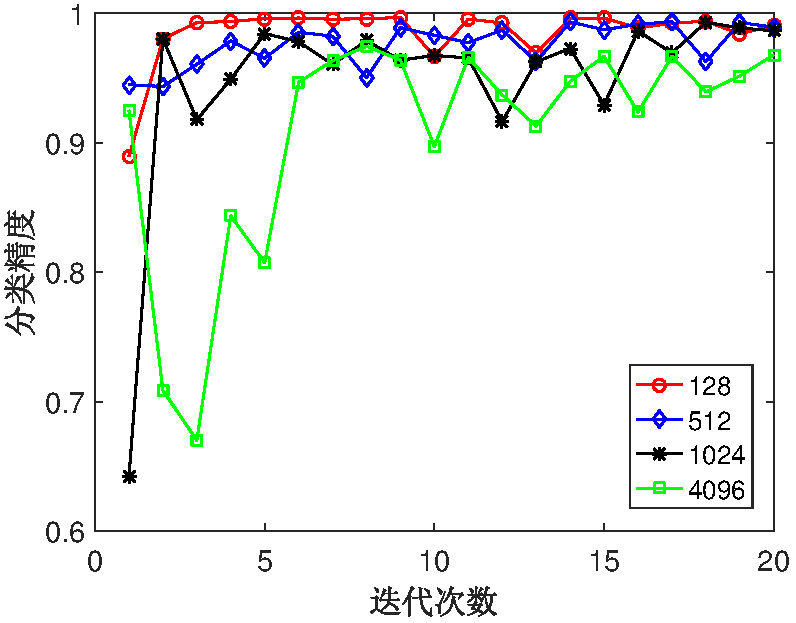
\includegraphics[width=6.67cm]{figures/othr/epoch}
	\caption{不同批长度下,分类准确度与迭代次数曲线图}
	\label{fig:epoch}
\end{figure}

在预处理阶段利用了滑窗算法对输入数据进行融合处理来减少由于某一帧数据中某距离方位单元上的随机噪声对识别结果的影响,此处对窗长参数变化对结果的影响进行测试比较。
主要考虑到电离层会随时间发生变化且天波雷达的采样周期较长,过长的窗长无法及时响应电离层的变化,影响识别准确率及与地图的匹配度。
为了选取一个合适的窗长,首先利用不同窗长平均融合后的数据进行测试,得到图\ref{fig:window}的结果,该结果证明了在窗长过长时,匹配度会下降的结论,当窗长过大时匹配度会降到比窗长为1时还要低。
为了进一步比较权重的变化对识别结果的影响,选取\equref{equ:window_fusion}中的权重为$w_N=\frac{1}{2},w_k=\frac{1}{2(N-1)},k=1,2,\dots,N-1$
,得到如图\ref{fig:weighted_window}所示的结果。
由于增加了主单元的权重,故在窗长增加时,匹配度没有明显下降。

\begin{figure}[hbt]
	\centering
	\begin{minipage}{7cm}
		\centering
		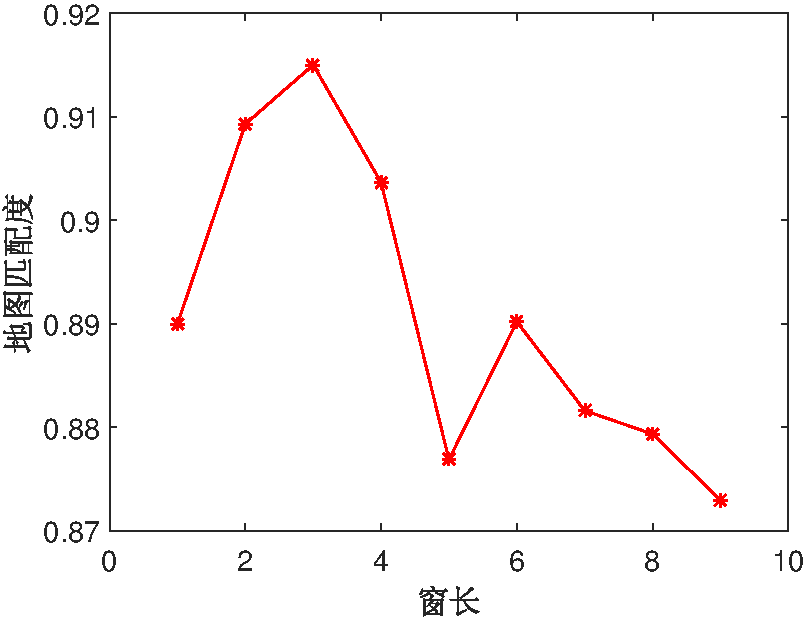
\includegraphics[width=6.67cm]{figures/othr/window}
		\caption{匹配度与融合窗长对比曲线图}
		\label{fig:window}
	\end{minipage}
	\hspace{10pt}
	\begin{minipage}{7cm}
		\centering
		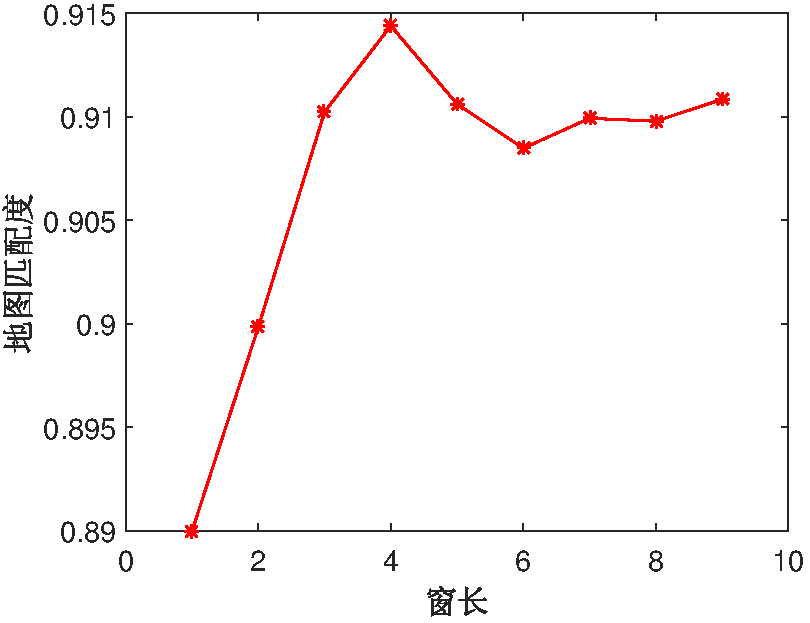
\includegraphics[width=6.67cm]{figures/othr/weighted_window}
		\caption{更改权重后不同窗长匹配度结果对比曲线图}
		\label{fig:weighted_window}
	\end{minipage}

\end{figure}


为了找出区分识别结果中海洋与陆地的最佳概率阈值,使用不同的概率阈值计算相同测试数据的正确率。图\ref{fig:threshold}显示,当阈值增大时,分类识别精度也随之提高,但精度的提高速度越来越慢,直至平稳。另一方面,当阈值仅为$0.01$时,识别率仍高于$0.86$。这说明本章方法的分类结果的概率值均处于较高的水平,如\ref{fig:prob}所示。

\begin{figure}[hbt]
	\centering
	\begin{minipage}{7cm}
		\centering
		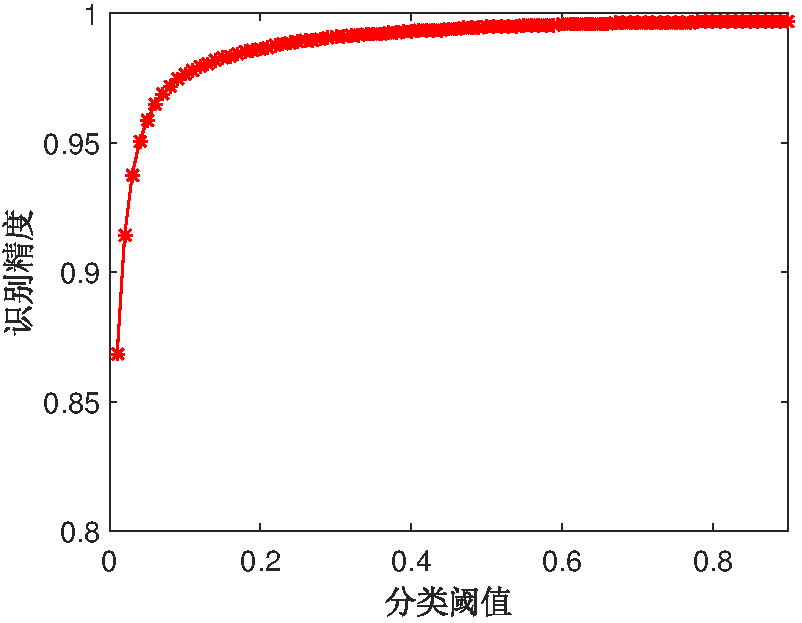
\includegraphics[width=6.67cm]{figures/othr/threashold}
		\caption{识别率与概率阈值曲线图}
		\label{fig:threshold}
	\end{minipage}
	\hspace{10pt}
	\begin{minipage}{7cm}
		\centering
		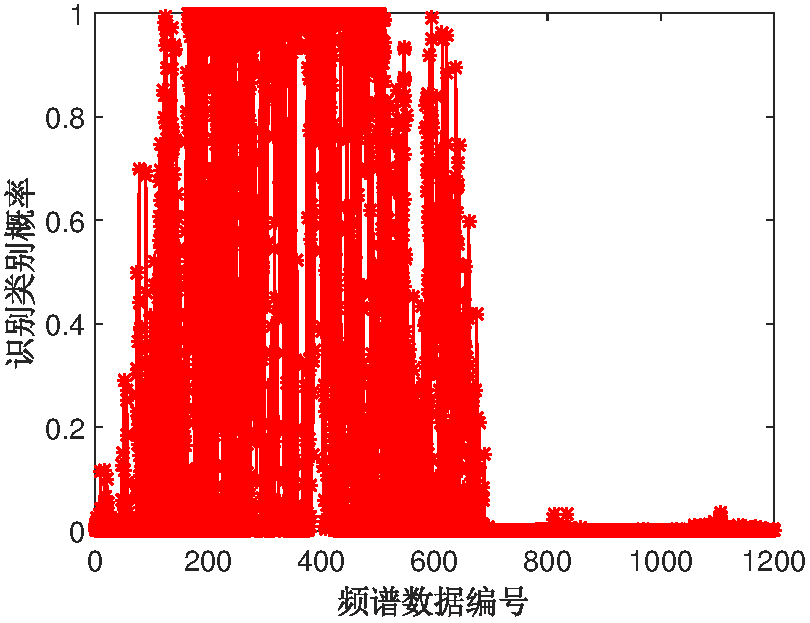
\includegraphics[width=6.67cm]{figures/othr/prob}
		\caption{不同帧数据识别结果概率值}
		\label{fig:prob}
	\end{minipage}

\end{figure}

为了验证提出的深度卷积神经网络地海杂波识别算法是否具有实时识别的能力,在CPU为i5-3.30GHz、运存为1GB的Linux虚拟机运行本章的算法程序,对整帧数据(共 20400 个分辨单元,每个分辨单元的相干积累点数为1024),其识别过程中占用内存峰值为178.5MB,识别时间为0.494141秒,其具备实时运行的能力。

% 经过上述在多个不同数据集上的实验,对我们的算法和基于支持向量机的识别算法和基于LMS的算法的对比分析,可以得到下述结论:
% \begin{itemize}
% 	\item 本章基于卷积神经网络的方法中获得最好的结果,且在地图匹配结果方面显著优于其余两种方法。
% 	\item 我们的方法具有很强的鲁棒性,雷达参数或者自然变化对识别结果影响不大。
% \end{itemize}

\subsection{特征可视化}
%TODO: \textcolor{red}{该部分需要添加详细的内容}

上一节利用大量测试数据的识别结果以及地图匹配结果对基于卷积神经网络的算法进行了验证,但是卷积神经网络方法有一个问题是其是黑盒操作,无法直观地看到其用于分类的特征。
因此,为了在理论上对本章算法的有效性进行分析。本节使用基于梯度变化的可视化方法,其思想为通过计算当输入数据的某个数据点发生变化时输出梯度的变化,得到每一个数据点对输出梯度的影响,从而得到该频谱数据热力图。
定义频谱数据序列为$ S = \{s_1, s_2, \dots,s_n\} $,其中$n$是频谱序列中的点数,设输出概率为$p(S)$。那么,可以得到\equref{equ:ps}:
\begin{equation}
	p(S) = w^TS+b,
	\label{equ:ps}
\end{equation}
其中$ w $和$ b $分别是模型的权重和偏差。实际上,权重$ w $表示对应点的重要性。在本章提出的模型中,类概率函数$p(S)$是高度非线性函数,可以使用泰勒方法近似$p(S)$。为了简化计算,使用一阶泰勒展开:
\begin{equation}
	w = \frac{\partial{p}}{\partial{S}}{\mid}_{s_i}.
	\label{equ:w}
\end{equation}

因此,可以通过反向传播计算得到$ w $的\equref{equ:w}。图\ref{fig:vis}显示,特征点主要集中在预期的数据上。
\begin{figure}[hbt]
%	\setlength{belowskip=-10pt}
	\setlength{\belowcaptionskip}{0pt}
	\centering
	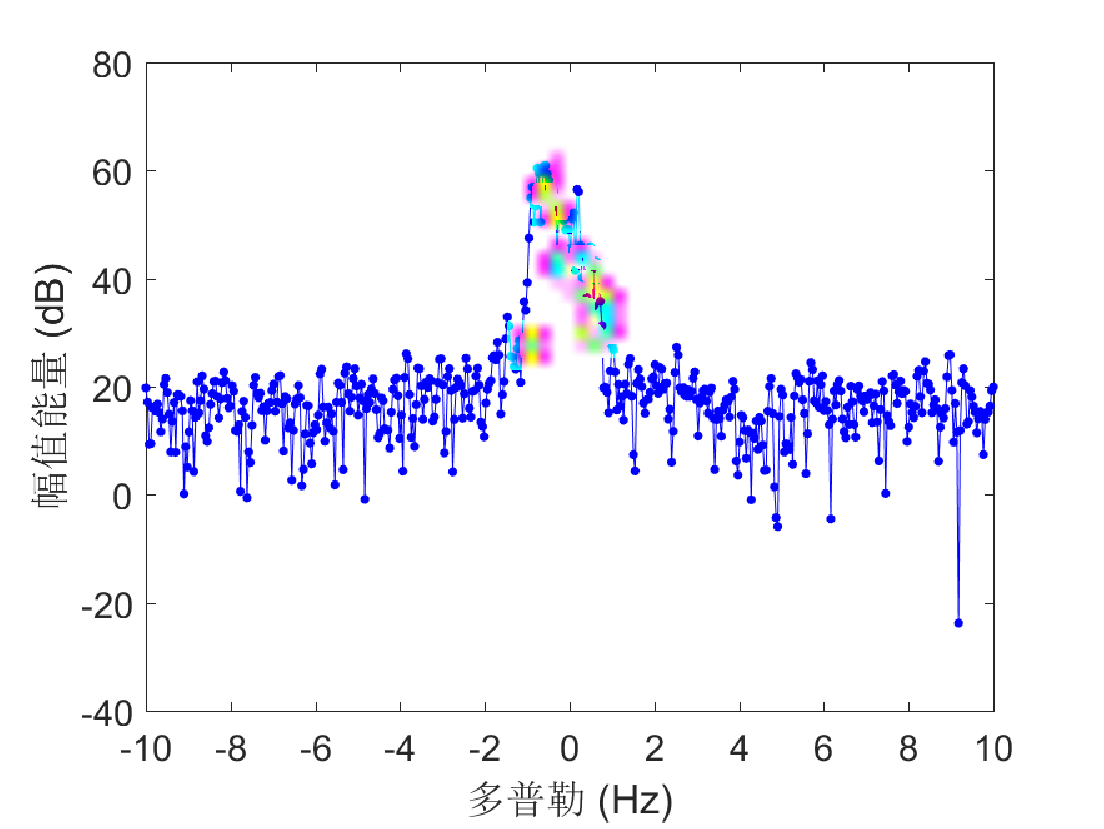
\includegraphics[width=6.67cm]{figures/othr/heatmap}
	\caption{特征重要程度热力图}
	\label{fig:vis}
\end{figure}

\section{小结}
\label{sec:othr_summary}
本章提出了基于卷积神经网络天波雷达地海杂波识别的新算法。该方法主要克服了基于LMS的方法或支持向量机算法根据经验从频谱数据中提取特征导致的操作复杂度高、分类精度低等缺点。通过与这两种算法进行了对比实验,结果表明本章提出的方法在地海杂波识别问题上更加有效且具有更强的抗干扰性能,且在地图匹配结果方面显著优于其余两种方法。
在更高精度的识别结果的帮助下,可以得到更加精确的修正系数,从而为目标定位问题提供更大的帮助。
% ,并利用同一区域不同时间的的频谱数据进行融合预处理
% 另一方面,如果我们针对于特定的问题对卷积神经网络的参数进行调整,可以进一步提高我们算法的性能。
